\documentclass[11pt]{article}
\usepackage{amssymb, amsthm, amsmath}
\usepackage{bm}
\usepackage{graphicx}
\usepackage[authoryear]{natbib}
\usepackage{bm}
\usepackage{verbatim}
\usepackage{lineno}
\usepackage{times}
\usepackage{soul}
\usepackage{color}
\usepackage{enumerate}
\usepackage{setspace}
\usepackage{times}
\usepackage{changepage}
\usepackage{multirow}

\usepackage[left=1in,top=1in,right=1in]{geometry}
\pdfpageheight 11in
\pdfpagewidth 8.5in
\linespread{2.0}
\newcommand{\btheta}{ \mbox{\boldmath $\theta$}}
\newcommand{\bmu}{ \mbox{\boldmath $\mu$}}
\newcommand{\balpha}{ \mbox{\boldmath $\alpha$}}
\newcommand{\bbeta}{ \mbox{\boldmath $\beta$}}
\newcommand{\bdelta}{ \mbox{\boldmath $\delta$}}
\newcommand{\blambda}{ \mbox{\boldmath $\lambda$}}
\newcommand{\bgamma}{ \mbox{\boldmath $\gamma$}}
\newcommand{\brho}{ \mbox{\boldmath $\rho$}}
\newcommand{\bpsi}{ \mbox{\boldmath $\psi$}}
\newcommand{\bepsilon}{ \mbox{\boldmath $\epsilon$}}
\newcommand{\bomega}{ \mbox{\boldmath $\omega$}}
\newcommand{\bOmega}{ \mbox{\boldmath $\Omega$}}
\newcommand{\bDelta}{ \mbox{\boldmath $\Delta$}}
\newcommand{\bSigma}{ \mbox{\boldmath $\Sigma$}}
\newcommand{\bPsi}{\mbox{\boldmath $\Psi$}}
\newcommand{\bOne}{\mbox{\boldmath $1$}}
\newcommand{\omu}{\overline{\mu}}
\newcommand{\oSigma}{\overline{\Sigma}}
\newcommand{\Yt}{{\tilde Y}}
\newcommand{\bA}{ \mbox{\bf A}}
\newcommand{\bP}{ \mbox{\bf P}}
\newcommand{\bx}{ \mbox{\bf x}}
\newcommand{\bX}{ \mbox{\bf X}}
\newcommand{\bB}{ \mbox{\bf B}}
\newcommand{\bT}{ \mbox{\bf T}}
\newcommand{\bZ}{ \mbox{\bf Z}}
\newcommand{\by}{ \mbox{\bf y}}
\newcommand{\bY}{ \mbox{\bf Y}}
\newcommand{\bz}{ \mbox{\bf z}}
\newcommand{\bh}{ \mbox{\bf h}}
\renewcommand{\bm}{ \mbox{\bf m}}
\newcommand{\br}{ \mbox{\bf r}}
\newcommand{\bt}{ \mbox{\bf t}}
\newcommand{\bk}{\mbox{\bf k}}
\newcommand{\bs}{ \mbox{\bf s}}
\newcommand{\bb}{ \mbox{\bf b}}
\newcommand{\bL}{ \mbox{\bf L}}
\newcommand{\bu}{ \mbox{\bf u}}
\newcommand{\bv}{ \mbox{\bf v}}
\newcommand{\bV}{ \mbox{\bf V}}
\newcommand{\bW}{ \mbox{\bf W}}
\newcommand{\bG}{ \mbox{\bf G}}
\newcommand{\bH}{ \mbox{\bf H}}
\newcommand{\bw}{ \mbox{\bf w}}
\newcommand{\bo}{ \mbox{\bf o}}
\newcommand{\bfe}{ \mbox{\bf e}}
\newcommand{\iid}{\stackrel{iid}{\sim}}
\newcommand{\ind}{\stackrel{ind}{\sim}}
\newcommand{\dd}{\; \text{d} }
\newcommand{\ddd}{\text{d} }
\newcommand{\indep}{\stackrel{indep}{\sim}}
\newcommand{\converged}{\stackrel{d}{\rightarrow}}
\newcommand{\goesto}[1]{\stackrel[#1]{}{\longrightarrow}}
\newcommand{\calR}{{\cal R}}
\newcommand{\calG}{{\cal G}}
\newcommand{\calD}{{\cal D}}
\newcommand{\calS}{{\cal S}}
\newcommand{\calB}{{\cal B}}
\newcommand{\calA}{{\cal A}}
\newcommand{\calT}{{\cal T}}
\newcommand{\calO}{{\cal O}}
\newcommand{\argmax}{{\mathop{\rm arg\, max}}}
\newcommand{\argmin}{{\mathop{\rm arg\, min}}}
\newcommand{\Frechet}{\mbox{Fr$\acute{\mbox{e}}$chet }}
\newcommand{\Matern}{\mbox{Mat$\acute{\mbox{e}}$rn }}
\newcommand{\ballunion}{B_a(\bs_1) \cup B_b(\bs_2) }

\newcommand{\alphahat}{\hat{\alpha}}

\newcommand{\eref}[1]{(\ref{#1})}
\newcommand{\fref}[1]{Figure~\ref{#1}}
\newcommand{\tref}[1]{Table~\ref{#1}}
\newcommand{\sref}[1]{Section~\ref{#1}}
\newcommand{\aref}[1]{Appendix~\ref{#1}}

\newcommand{\beq}{ \begin{equation}}
\newcommand{\eeq}{ \end{equation}}
\newcommand{\beqn}{ \begin{eqnarray}}
\newcommand{\eeqn}{ \end{eqnarray}}

\newcommand*\patchAmsMathEnvironmentForLineno[1]{%
  \expandafter\let\csname old#1\expandafter\endcsname\csname #1\endcsname
  \expandafter\let\csname oldend#1\expandafter\endcsname\csname end#1\endcsname
  \renewenvironment{#1}%
     {\linenomath\csname old#1\endcsname}%
     {\csname oldend#1\endcsname\endlinenomath}}% 
\newcommand*\patchBothAmsMathEnvironmentsForLineno[1]{%
  \patchAmsMathEnvironmentForLineno{#1}%
  \patchAmsMathEnvironmentForLineno{#1*}}%
\AtBeginDocument{%
\patchBothAmsMathEnvironmentsForLineno{equation}%
\patchBothAmsMathEnvironmentsForLineno{align}%
\patchBothAmsMathEnvironmentsForLineno{flalign}%
\patchBothAmsMathEnvironmentsForLineno{alignat}%
\patchBothAmsMathEnvironmentsForLineno{gather}%
\patchBothAmsMathEnvironmentsForLineno{multline}%
}



\begin{document}\linenumbers
\pagestyle{empty}
\begin{center}
{\Large {\bf Exploration and inference in spatial extremes using empirical basis functions}}\\

{\large Samuel A Morris\footnote[1]{North Carolina State University}, Brian J Reich\footnotemark[1]{}, and Emeric Thibauld\footnote[2]{Colorado State University}}

%\footnote{This is the footnote} looks like this. Later text referring to same footnote\footnotemark[\value{footnote}]
\today
\end{center}


\begin{abstract}
	words...\\
	{\bf Key words}: Bayesian data analysis; principal components analysis; max-stable process; spectral representation.

\end{abstract}
\newpage
\pagestyle{plain}
\setcounter{page}{1}

\section{Introduction}\label{ebs:intro}
The spatial Extreme Value Analysis (EVA) literature is expanding rapidly \citep{Davison2012} to meet the demands of researchers to improve estimates of rare-event probabilities by borrowing information across space and to estimate the probability of extreme events occurring simultaneously at multiple locations.
Environmental datasets commonly include observations from hundreds or thousands of locations, and advanced tools are required to explore and analyze these data.
For Gaussian data, Principle Components Analysis \citep[PCA]{Everitt2008}, also known as Empirically Orthogonal Functions \citep[EOF]{Toggweiler2001}, has proven to be a powerful tool to study correlation between spatial locations; understand the most important large-scale spatial features; and reduce the dimension of the problem to allow for simple computation even for massive datasets.
Computation and exploration is arguably more difficult for EVA than Gaussian data, yet to our knowledge no tool analogous to spatial PCA has been developed for EVA.

In EVA, extremes are separated from the bulk of the distribution by either analyzing only points above a threshold or block maximums \citep{Coles2001}, e.g., the annual maximum of the daily precipitation.
A natural spatial model for block maximum at several spatial locations is the max-stable process, which, under certain conditions, arises as the limit of the location-wise maximum of infinitely-many spatial processes \citep{deHaan2006}.
\Citet{deHaan1984} showed that any max-stable process can be represented in terms of a countable number of spatial processes (e.g., stationary log Gaussian processes), and a finite truncation of this representation has been used for conditional simulation \citep{Wang2011}.
The proposed EBF approach also uses a finite truncation of the spectral representation, and develops a method-of-moments estimator for the underlying spatial processes.

In addition to exploratory analysis, we show that the EBFs can be used for Bayesian inference on the marginal parameters at each location and to test for covariate effects.
Fully-Bayesian analysis using max-stable processes is cumbersome for large data sets \citep{Wadsworth2014,Thibaud2013a}.
One option is to use non-max-stable models that retain extremal dependence such as the skew-t process in Morris et al \hl{put on arxiv}.
Alternatively, \citet{Reich2012} propose a low-rank method based on spatial kernel functions, and others have used pairwise \citep{Padoan2010,Huser2014} and trivariate \citep{Genton2011} likelihood methods for parameter estimation.

In this paper we develop methodology to use the spectral representation of a max-stable process to identify a small set of empirical basis functions (EBF) that capture the most important spatial features of the data.
Unlike PCA/EOFs, the EBFs are not orthogonal, nonetheless these spatial functions can be plotted for exploratory analysis to reveal important spatial trends.
The EBFs can also be used in a second-stage statistical analysis.
By basing the spatial dependence on EBFs, the resulting spatial analysis does not require dubious assumptions such as stationarity.
In addition, a Bayesian analysis for either block-maximum or point above a threshold is computationally feasible for large datsets because the entire spatial process is represented by a small number of basis functions.

The paper proceeds as follows. In \sref{ebs:model} we present the low-rank model. \hl{More here about the sections}

\section{Model}\label{ebs:model}

Let $Y_{t}(\bs)$ be the observation at spatial location $\bs$ and time $t$.  We temporarily drop the subscript $t$ and describe the model for the process $Y(\bs)$ for a single time point, but return to the spatiotemporal setting in \sref{ebs:estimation}.
To focus attention on the extreme values, we emphasize the statistical model for exceedances above a location-specific threshold $T(\bs)$.
We begin by specifying a spatial model for the complete data $Y(\bs)$ and then use the censored likelihood defined by $T(\bs)$ for inference as described in \sref{ebs:MCMC}.
Although the model presented implements a censored likelihood, the model also can fit uncensored data (such as block-maxima) by setting $T(\bs) = -\infty$.

Spatial dependence is captured by modeling $Y(\bs)$ as a max-stable process \citep{deHaan2006}.
Max-stable processes have generalized extremal value (GEV; see Appendix A.1) marginal distribution.
The GEV has three parameters: location $\mu(\bs)$; scale $\sigma(\bs)$; and shape $\xi(\bs)$.
Spatial dependence is present both in the GEV parameters but also the standardized residual process
\beq\label{ebeq:Y2Z}
 Z(\bs) = \left\{1+\frac{\xi(\bs)}{\sigma(\bs)}\left[Y(\bs) - \mu(\bs)\right]\right\}^{1/\xi(\bs)},
\eeq which has unit $\Frechet$ (i.e., GEV with location, scale, and shape all equal one) marginal distribution for all $\bs$.

Our objective is to identify a low-rank model for the spatial dependence of $Z(\bs)$.
The spectral representation theorem \citep{deHaan1984} states that any max-stable process can be written
\beq\label{ebeq:spectral}
  Z(\bs) = \mbox{sup}_l B(\bs,\bt_l)A_{l}
\eeq
where the function $B$ satisfies $B(\bs,\bt)>0$ for all $(\bs,\bt)$ and $\int B(\bs,\bt)d\bt=1$ for all $\bs$, and $(\bt_l,A_l)$ for $l=1,...,\infty$ are a Poisson process with intensity measure $dA d\bt/A^2$.

We follow \citet{Reich2012} and decompose  $Z(\bs)$ as $Z(\bs)=\theta(\bs)\varepsilon(\bs)$ where $\theta(\bs)$ is a spatial process and $\varepsilon(\bs)\iid$ GEV$(1,\alpha,\alpha)$ is independent error.
The spatial component is
\beq \label{ebeq:theta}
  \theta(\bs) = \left(\sum_{l=1}^LB_{l}(\bs)^{1/\alpha}A_{l}\right)^{\alpha}.
\eeq
If $B_{l}(\bs)>0$, $\sum_{l=1}^LB_{l}(\bs)=1$ for all $\bs$, and the $A_{l}$ have positive stable (PS; Appendix A.1) distribution $A_{l}\iid$ PS$(\alpha)$, then $Z(\bs)$ is max-stable and has unit $\Frechet$ marginal distributions.

Extremal spatial dependence can be summarized by the extremal coefficient \citep[EC]{Schlather2003} $\vartheta(\bs,\bt)\in[1,2]$, where
\beq\label{ebeq:ECdev}
  \mbox{Prob}[Z(\bs)<c,Z(\bt)<c] = \mbox{Prob}[Z(\bs)<c]^{\vartheta(\bs,\bt)}.
\eeq
For the PS random effects model the EC has the form
\beq\label{ebeq:EC}
   \vartheta(\bs,\bt) = \sum_{l=1}^L \left[B_{l}(\bs)^{1/\alpha}+B_{l}(\bs)^{1/\alpha}\right]^\alpha.
\eeq
In particular, $\vartheta(\bs,\bs) = 2^{\alpha}$ for all $\bs$.

\section{Estimating the spatial dependence function}\label{ebs:estimation}

To estimate the extremal coefficient function, we consider the process at $n_s$ spatial locations $\bs_1,...,\bs_{n_s}$ and $n_t$ times $t=1,...,n_t$.
Denote $Y_t(\bs_i) = Y_{it}$, $B_l(\bs_i) = B_{il}$, $T(\bs_i)=T_i$, and $\vartheta(\bs_i,\bs_j) = \vartheta_{ij}$.
In this section we develop an algorithm to estimate the spatial dependence parameter $\alpha$ and the $n_s\times L$ matrix $\bB = \{B_{il}\}$.
Given these parameters, we insert them into our model and proceed with Bayesian analysis as described in \sref{ebs:MCMC}.
Our algorithm has the following steps:
\begin{enumerate}[(1)]
  \item Obtain an initial estimate of the extremal coefficient for each pair of locations, ${\hat \vartheta}_{ij}$.
  \item Spatially smooth these initial estimates ${\hat \vartheta}_{ij}$ using kernel smoothing to obtain ${\tilde \vartheta}_{ij}$.
  \item Estimate the spatial dependence parameters by minimizing the difference between model-based coefficients, $\vartheta_{ij}$, and smoothed coefficients, ${\tilde \vartheta}_{ij}$.
\end{enumerate}

% Use for thesis
% The first-stage estimates are obtained using an empirical estimate as follows.
% To estimate the spatial dependence we first remove variation in the marginal distribution.
% Let $U_{it} = \sum_{k=1}^{n_t} I[Y_{ik}<Y_{it}]/n_t$, so that the $U_{it}$ are approximately uniform at each location.
% Then for some extreme probability $q\in(0,1)$, solving \eref{ebeq:ECdev} suggests the estimate
% \beq\label{ebeq:EChat0}
%    {\hat \vartheta}_{ij}(q) = \frac{\log[Q_{ij}(q)]}{\log(q)},
% \eeq
% where $Q_{ij}(q) = \sum_{t=1}^{n_t}I[U_{it}<q,U_{jt}<q]/n_t$ is the sample proportion of the time points at which both sites are less than $q$.
% Since all large $q$ give valid estimates, we average over a grid of $q$ with $q_1<...<q_{n_q}$
% \beq\label{ebeq:EChat1}
% {\hat \vartheta}_{ij} = \frac{1}{n_q}\sum_{j=1}^{n_q}{\hat \vartheta}_{ij}(q_j).
% \eeq

% Use for paper
The first-stage estimates are obtained using the \texttt{fitextcoeff} function in the \texttt{SpatialExtremes} package of \texttt{R}  using the \texttt{fitextcoeff} function in the \texttt{SpatialExtremes} \citep{Ribatet2015} package of \texttt{R} \citep{Rmanual}.
Assuming the true EC is smooth over space, the initial estimates ${\hat \vartheta}_{ij}$ can be improved by smoothing.
Let
\beq\label{ebeq:EChat2}
  {\tilde \vartheta}_{ij} = \frac{\sum_{u=1}^{n_s}\sum_{v=1}^{n_s} w_{iu}w_{jv}{\hat \vartheta}_{uv}}
  {\sum_{u=1}^{n_s}\sum_{v=1}^{n_s} w_{iu}w_{jv}},
\eeq
where $w_{iu} = \exp[-(||\bs_i-\bs_u'||/\phi)^2])$ is the Gaussian kernel function with bandwidth $\phi$.
The elements ${\hat \vartheta}_{ii}$ do not contribute any information as ${\hat \vartheta}_{ii}=1$ for all $i$ by construction.
To eliminate the influence of these estimates we set $w_{ii}=0$.
However, this approach does give imputed values ${\tilde \vartheta}_{ii}$, which provide information about small-scale spatial variability.

The dependence parameters are estimated by comparing estimates ${\tilde \vartheta}_{ij}$ with the model-based values $\vartheta_{ij}$.
For all $i$, $\vartheta_{ii} = 2^{\alpha}$, and therefore we set $\alpha$ to $\alphahat = \log_2(\sum_{i=1}^{n_s}{\tilde \vartheta}_{ii}/n_s)$.
Given $\alpha=\alphahat$, it remains to estimate $\bB$.
Following \citet{Smith1990}, we use squared-error loss, so the estimate $\hat{\bB}$ is the minimizer of
\beq\label{ebeq:Bhat}
\sum_{i<j} \left({\tilde \vartheta}_{ij} - \vartheta_{ij}\right)^2
  =
  \sum_{i<j} \left({\tilde \vartheta}_{ji} - \sum_{l=1}^L[B_{il}^{1/\alphahat} + B_{jl}^{1/\alphahat}]^{\alphahat}\right)^2
\eeq
under the restrictions that $B_{il}\ge 0$ for all $i$ and $l$ and $\sum_{l=1}^LB_{il}=1$ for all $i$.
Since the minimizer of \eref{ebeq:Bhat} does not have a closed form, we use block coordinate descent to obtain ${\hat \bB}$.
We cycle through spatial locations and update the vectors $(B_{i1},...,B_{iL})$ conditioned on the values for the other location and repeat until convergence.
At each step, we use the restricted optimization routine in the \texttt{R} function \texttt{optim}.
This algorithm gives estimates of the $B_{il}$ at the $n_s$ data locations, but is easily extended to all $\bs$ for spatial prediction.
The kernel smoothing step ensures that the estimates for $\hat{B}_{il}$ are spatially smooth, and thus interpolation of the $\hat{B}_{il}$ gives spatial functions $\hat{B}_l(\bs)$.

These functions provide useful exploratory data analysis techniques.
Maps of $\hat{B}_l(\bs)$ show important spatial features in the extremal dependence.
Furthermore, they allow for a non-stationary spatial dependence structure.
The relative contribution of each term can be measured by
\beq\label{ebeq:v}
v_l = \frac{1}{n_s}\sum_{i=1}^{n_s}{\hat B}_{il}.
\eeq
Since $\sum_{l=1}^L{\hat B}_{il}=1$ for all $i$, we have $\sum_{l=1}^Lv_l = 1$.
Therefore, terms with large $v_l$ are the most important.
The order of the terms is arbitrary, and so we reorder the terms so that $v_1\ge...\ge v_L$.

\section{Bayesian implementation details}\label{ebs:MCMC}
For our data analysis in \sref{ebs:analysis} we allow the GEV location and scale parameters, denoted $\mu_t(\bs)$ and scale $\sigma_t(\bs)$ respectively, to vary with space and time.
The model we choose is as follows
\begin{align}\label{ebeq:GPprior}
  \mu_t(\bs) &= \beta_{\mu, \text{int}}(\bs) + \beta_{\mu, \text{time}}(\bs) t\\
  \log[\sigma_t(\bs)] &= \beta_{\sigma, \text{int}}(\bs) + \beta_{\sigma, \text{time}}(\bs) t
\end{align}
where $\beta_{\mu, \text{int}}(\bs)$, $\beta_{\mu, \text{time}}(\bs)$, $\beta_{\sigma, \text{int}}(\bs)$, $\beta_{\sigma, \text{time}}(\bs)$ each have independent Gaussian process priors with an exponential spatial correlation matrix obtained from $\rho(h) = \exp\{- \frac{h}{\phi}\}$ where $h = ||\bs_1 - \bs_2||$ is the Euclidean distance between sites $\bs_1$ and $\bs_2$.
The GEV shape parameter $\xi$ is held constant over space and time because this parameter is notoriously difficult to estimate \hl{Emeric, do you happen to know a good reference here?}.
Collectively, let the marginal GEV parameters at location $i$ and time $t$ be $\Theta_{it} = \{\mu_{it},\sigma_{it},\xi\}$ where $\mu_{it} = \mu_t(\bs_i)$ and $\sigma_{it} = \sigma_t(\bs_i)$.

As shown in \citet{Reich2012}, the uncensored responses $Y_{t}(\bs)$ are conditionally independent given the spatial random effects, with conditional distribution
\beq\label{ebeq:Ycond}
   Y_{it}|\theta_{it},\Theta_{it}\indep GEV(\mu^*_{it}, \sigma_{it}^*,\xi^*),
\eeq
where $\mu_{it}^* = \mu_{it} + \frac{\sigma_{it}}{\xi}(\theta_{it}^\xi - 1)$,
$\sigma_{it}^* = \alpha\sigma_{it}\theta_{it}^\xi$, and $\xi^* = \alpha\xi$.
Therefore, the conditional likelihood conveniently factors across observations; marginalizing over the random effect $\theta_{it}$ induces extremal spatial dependence.
To focus on the extreme values above the local threshold $T_i$, we use the censored likelihood
\beq\label{ebeq:g}
d(y;\theta_{it},\Theta_{it}, T_i)  =
\left\{\begin{array}{ll}
    F(y;\mu_{it}^*,\sigma_{it}^*,\xi^*) & y \le T_i \\
  f(y;\mu_{it}^*,\sigma_{it}^*,\xi^*) & y>T_i,
\end{array}\right.
\eeq
where $F$ and $f$ are the GEV distribution and density functions, respectively, defined in Appendix A.1.

\hl{}
In summary, given the estimates of $\alpha$ and $\bB$, the hierarchical model is
\beqn \label{ebeq:bayesmodel}
  Y_{it} |\theta_{ij} & \indep & d(y;\theta_{it},\Theta_{it}, T_i) \\
  \theta_{it} &=& \left(\sum_{l=1}^L{\hat B}_{il}^{1/\alphahat}A_{lt}\right)^{\alphahat}
  \mbox{\ \ \ where \ \ \ }
  A_{lt} \iid PS(\alphahat)\nonumber\\
  \mu_{it} &=& \bX_{it}^\top \bbeta_1
  \mbox{\ \ \ and \ \ \ }
  \mbox{log}(\sigma_{it}) = \bX_{it}^\top \bbeta_2. \nonumber
\eeqn
\hl{I still need to finish updating this paragraph}
To complete the Bayesian model, we select independent normal priors with mean zero and variance $\sigma^2_1$ and $\sigma^2_2$ for the components of $\bbeta_1$ and $\bbeta_2$ respectively, and $\xi\sim \mbox{Normal}(0,0.5^2)$.
We use InvGamma(1, 1) priors for $\sigma^2_1$ and $\sigma^2_2$.
We estimate parameters $\Theta = \left\{A_{lt}, \bbeta_1, \bbeta_2, \xi, \sigma^2_1, \sigma^2_2 \right\}$ using Markov chain Monte Carlo methods.
We use a Metropolis-Hastings algorithm to update the model parameters with random walk candidate distributions for all parameters except $\sigma^2_1$ and  $\sigma^2_2$ which we update using Gibbs sampling.
The PS density is challenging to evaluate as it does not have a closed form.
One technique to avoid this complication is to incorporate auxiliary random variables \citep{Stephenson2009}, but we opt for a numerical approximation to the integral as described in Appendix \hl{still need to add this}.

The first-stage estimate of the extremal coefficients has three tuning parameters: the quantile thresholds $q_1,...,q_{n_q}$, the kernel bandwidth $\phi$, and the number of terms $L$.
In \sref{ebs:analysis} we explore a few possibilities for $\phi$ and $L$ and discuss sensitivity to these choices.
The second-stage Bayesian analysis requires selecting thresholds $T_i,...,T_{n_s}$.  For this we use spatially smoothed sample quantiles.
That is, we set $T_i$ to the 0.95 quantile of the $Y_{it}$ and its five nearest neighbors.

\section{Data analysis}\label{ebs:analysis}
In this section, we illustrate our method using both points above a threshold and block maxima.
In \sref{ebs:georgia}, we present an analysis using annual acreage burned due to wildfires in Georgia from 1965 -- 2014.
This is followed in \sref{ebs:precip} by an analysis of precipitation data in the eastern U.S.

\subsection{Analysis of extreme Georgia fires}\label{ebs:georgia}
The dataset used for our application is composed of yearly acreage burned due to wildfires for each county in Georgia from 1965 -- 2014 (\texttt{http://weather.gfc.state.ga.us/FireData/}).
\fref{ebfig:firets25} shows the time series of $\log$(acres burned) for 25 randomly selected counties.
Based on this plot and other exploratory analysis, we see no evidence of non-linear trends and proceed with linear time trends for the GEV location and scale parameters.
For covariates we use the standardized linear time trend $t^* = (t-n_t/2)/n_t$, and $L$ bivariate Gaussian kernel functions $\widetilde{B}_{il}$, and their interactions: $\bX_{it} = (1,t^*,\widetilde{B}_{i1},...,\widetilde{B}_{iL},t^*\widetilde{B}_{i1},...,t^*\widetilde{B}_{iL})^\top$.
For the bivariate Gaussian kernels, we select $L$ knot locations, $\bv_{1}, \ldots, \bv_{L}$ from the county centroids, using a space-filling design (\hl{ref add to bibtex Johnson, M.E., Moore, L.M., and Ylvisaker, D. ,1990}).
Then
\begin{align}\label{ebeq:bivGausskern}
  \widetilde{B}_{il} = \exp\left\{-\frac{||\bs_i - \bv_l||^2}{\rho^2}\right\}
\end{align}
where $\rho$ is included as an unknown parameter with a U($\rho_l$, $\rho_u$) prior where $\rho_l$ is the 5th quantile of $||\bs_i - \bv_l||^2$ and $\rho_u$ is the 95th quantile of $||\bs_i - \bv_l||^2$ \hl{basically I took the 5th and 95th quantile of the squared distances between the sites and the knots}.


\vspace{2em} % remove this

\begin{figure}[htbp]  % markdown/eda/eda-plotting.R
  \centering
  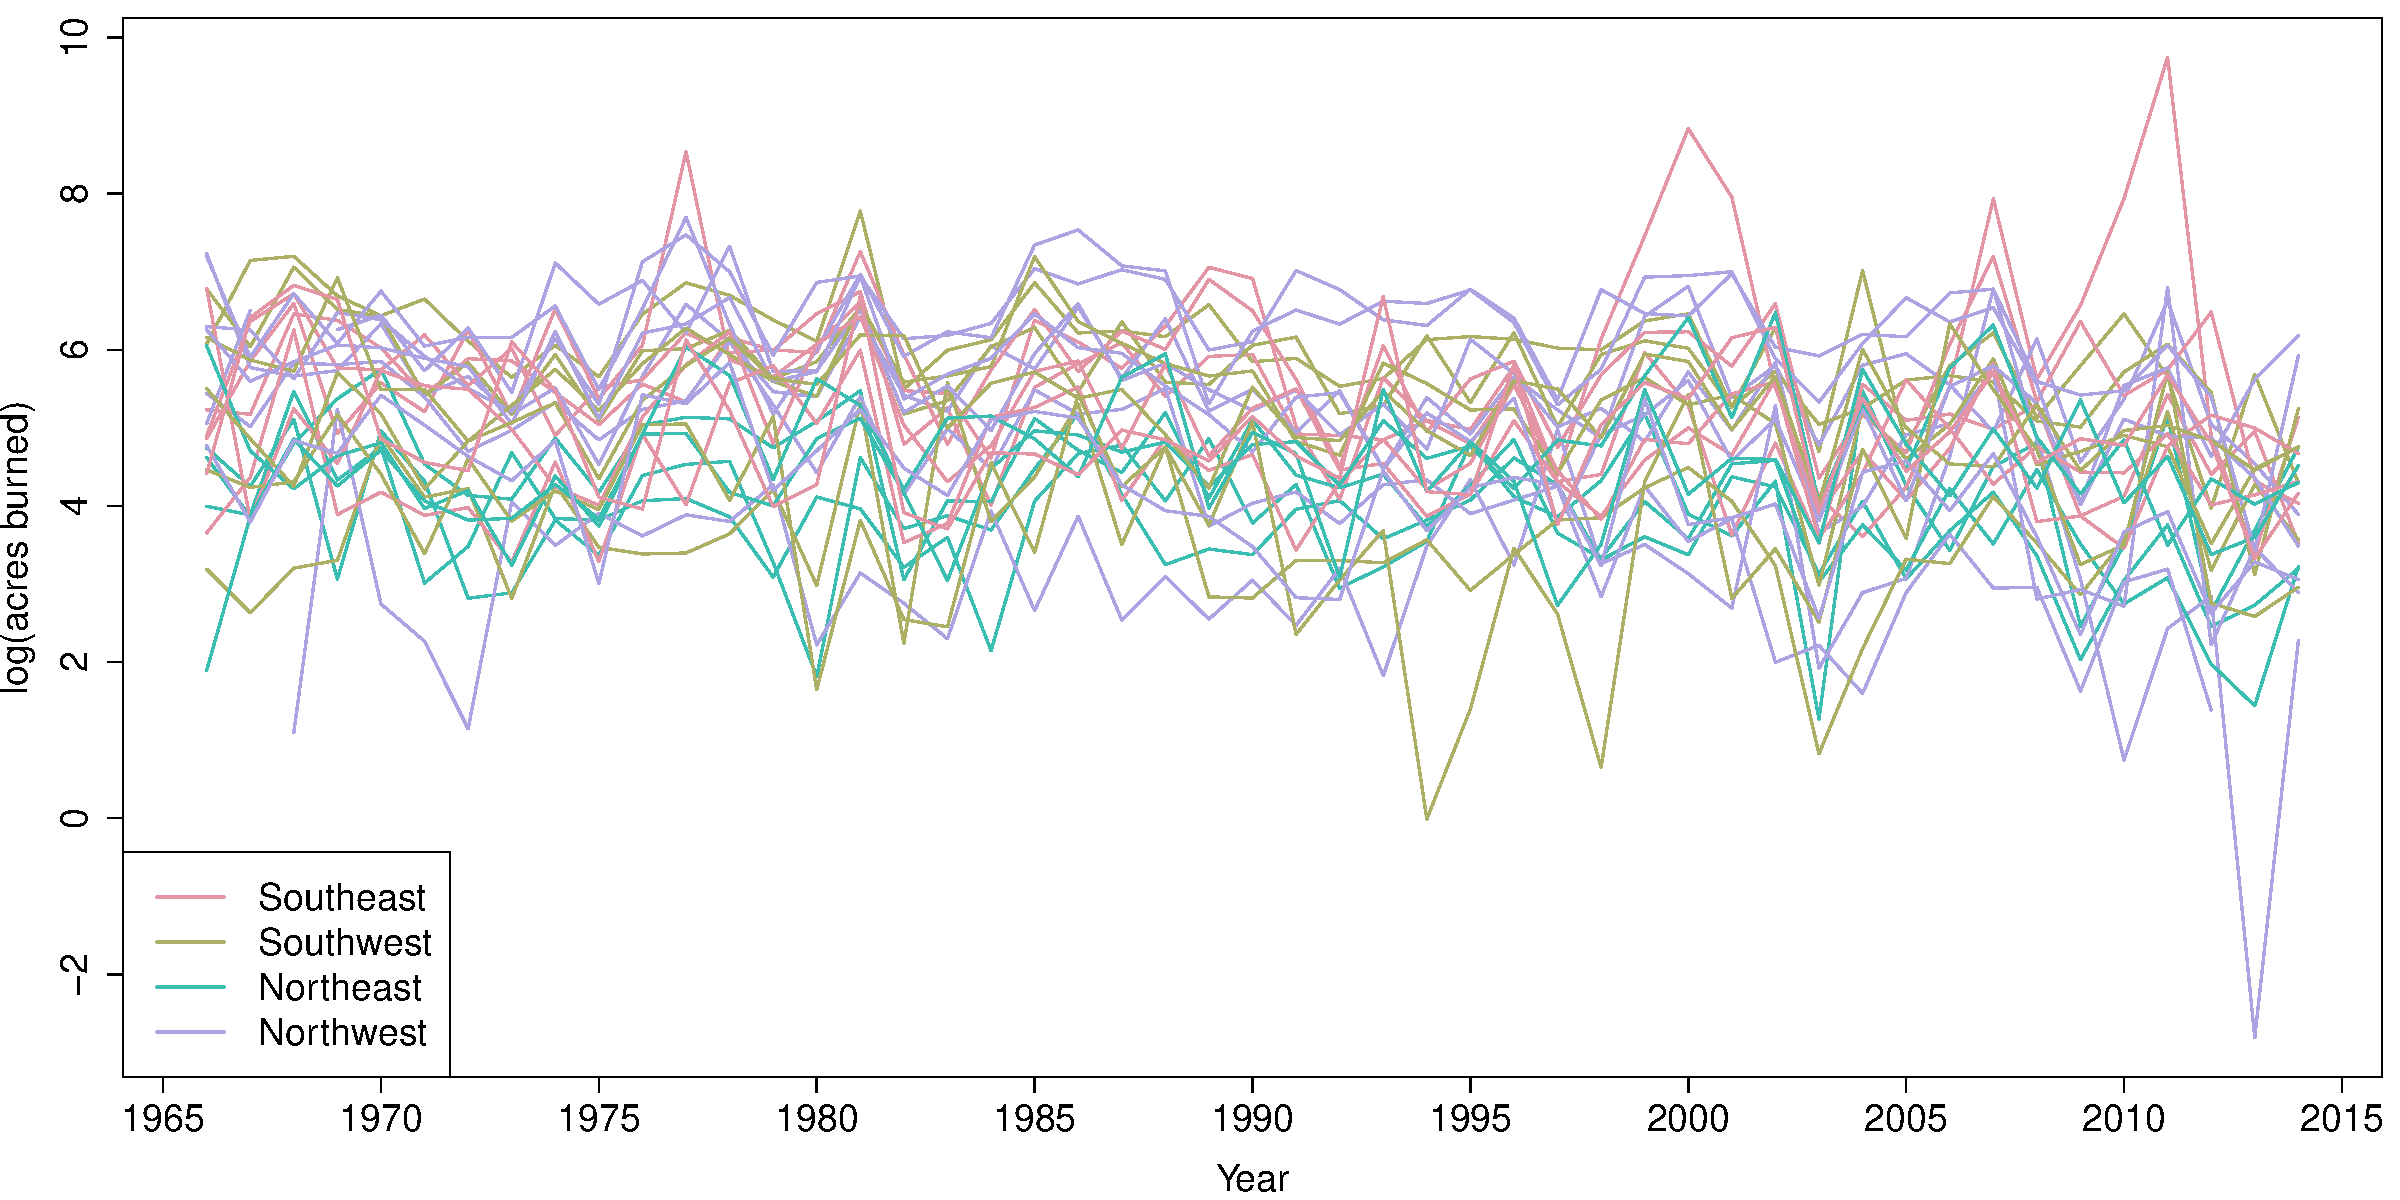
\includegraphics[width=0.47\linewidth]{plots/fire-spag-rand-25}
  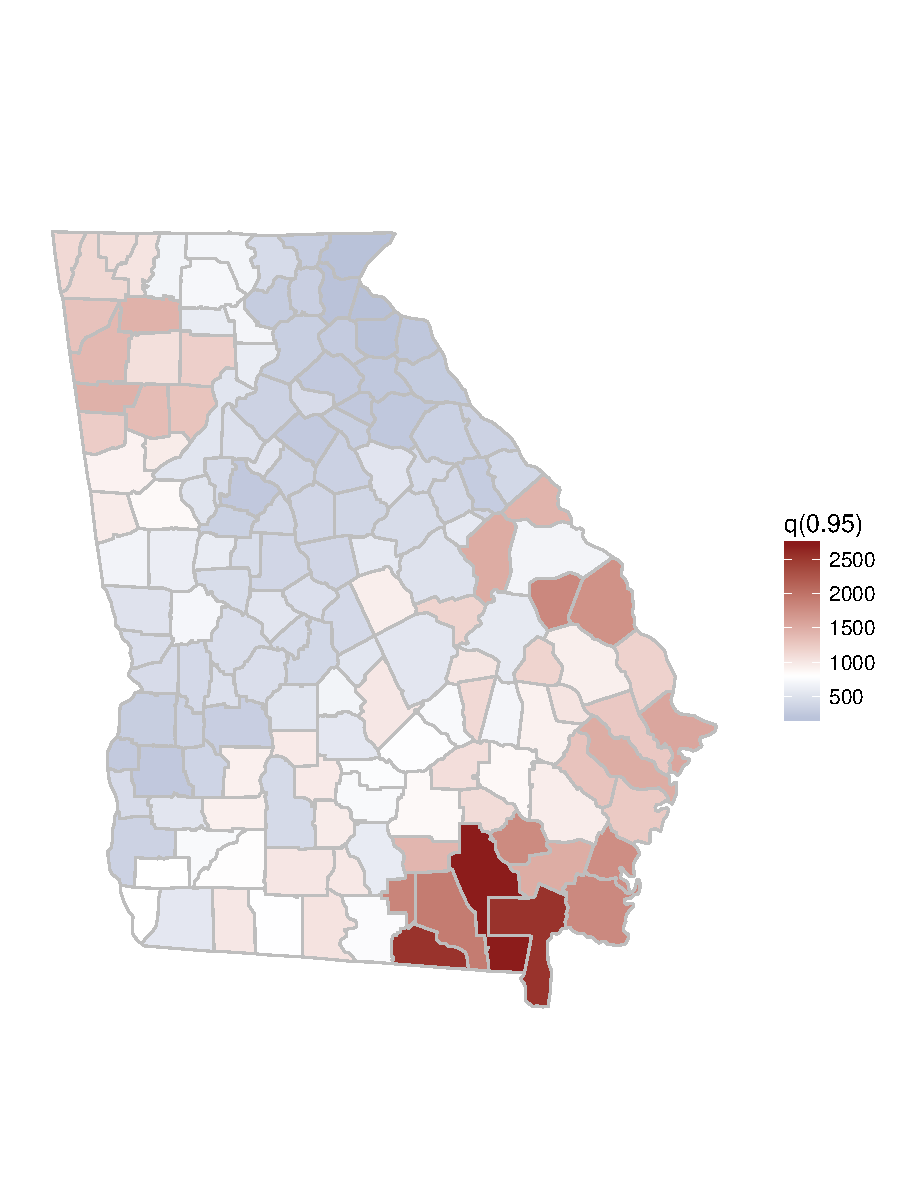
\includegraphics[width=0.47\linewidth, trim = 0 10em 0 10em]{plots/fire-spatial-q95.pdf}
  \caption{Time series of log acres burned for 25 randomly selected counties with colors coding the county's quadrant (left), and spatially smoothed threshold values, $T_i$ for each county (right).}
  \label{ebfig:firets25}
\end{figure}

We estimate the extremal coefficient function $\hat{\theta}_{ij}$ by setting $q_1 = 0.90$ and using $n_q = 100$.
With more data, it would possible to increase $q_1$, but we set $q_1 = 0.90$ to increase the stability when estimating $\hat{\vartheta}_{ij}$.

Because these data are not block-maxima, we select a site-specific threshold $T_i$ to use in the analysis with the following algorithm.
Without some adjustment to the data, it is challenging to borrow information across sites to inform the threshold selection.
We first standardize the data, separated by county, by subtracting the site's median and dividing by the site's interquartile range.
Denote the standardized data by $\widetilde{\bY}_i$.
% \begin{align}
%   \widetilde{\bY}_i = \frac{\bY_i - \text{med}(\bY_i)}{\text{IQR}(\bY_i)}
% \end{align}
% where med$(\cdot)$ is the median, and IQR$(\cdot)$ is the inter-quartile range.
Then we combine all sites together and plot a mean residual plot for $\widetilde{Y}_{it}, i = 1, \ldots, n_s$ and $t = 1, \ldots, n_t$.
The mean residual plot is given in \fref{ebfig:mrlthresh}.
Based upon the mean residual plot, we select the 95th percentile for the threshold.
To calculate $T_i$ for each county, we use the 95th percentile for the combined data for county $i$ and its five closest counties.

\begin{figure}[htbp]
  \centering
  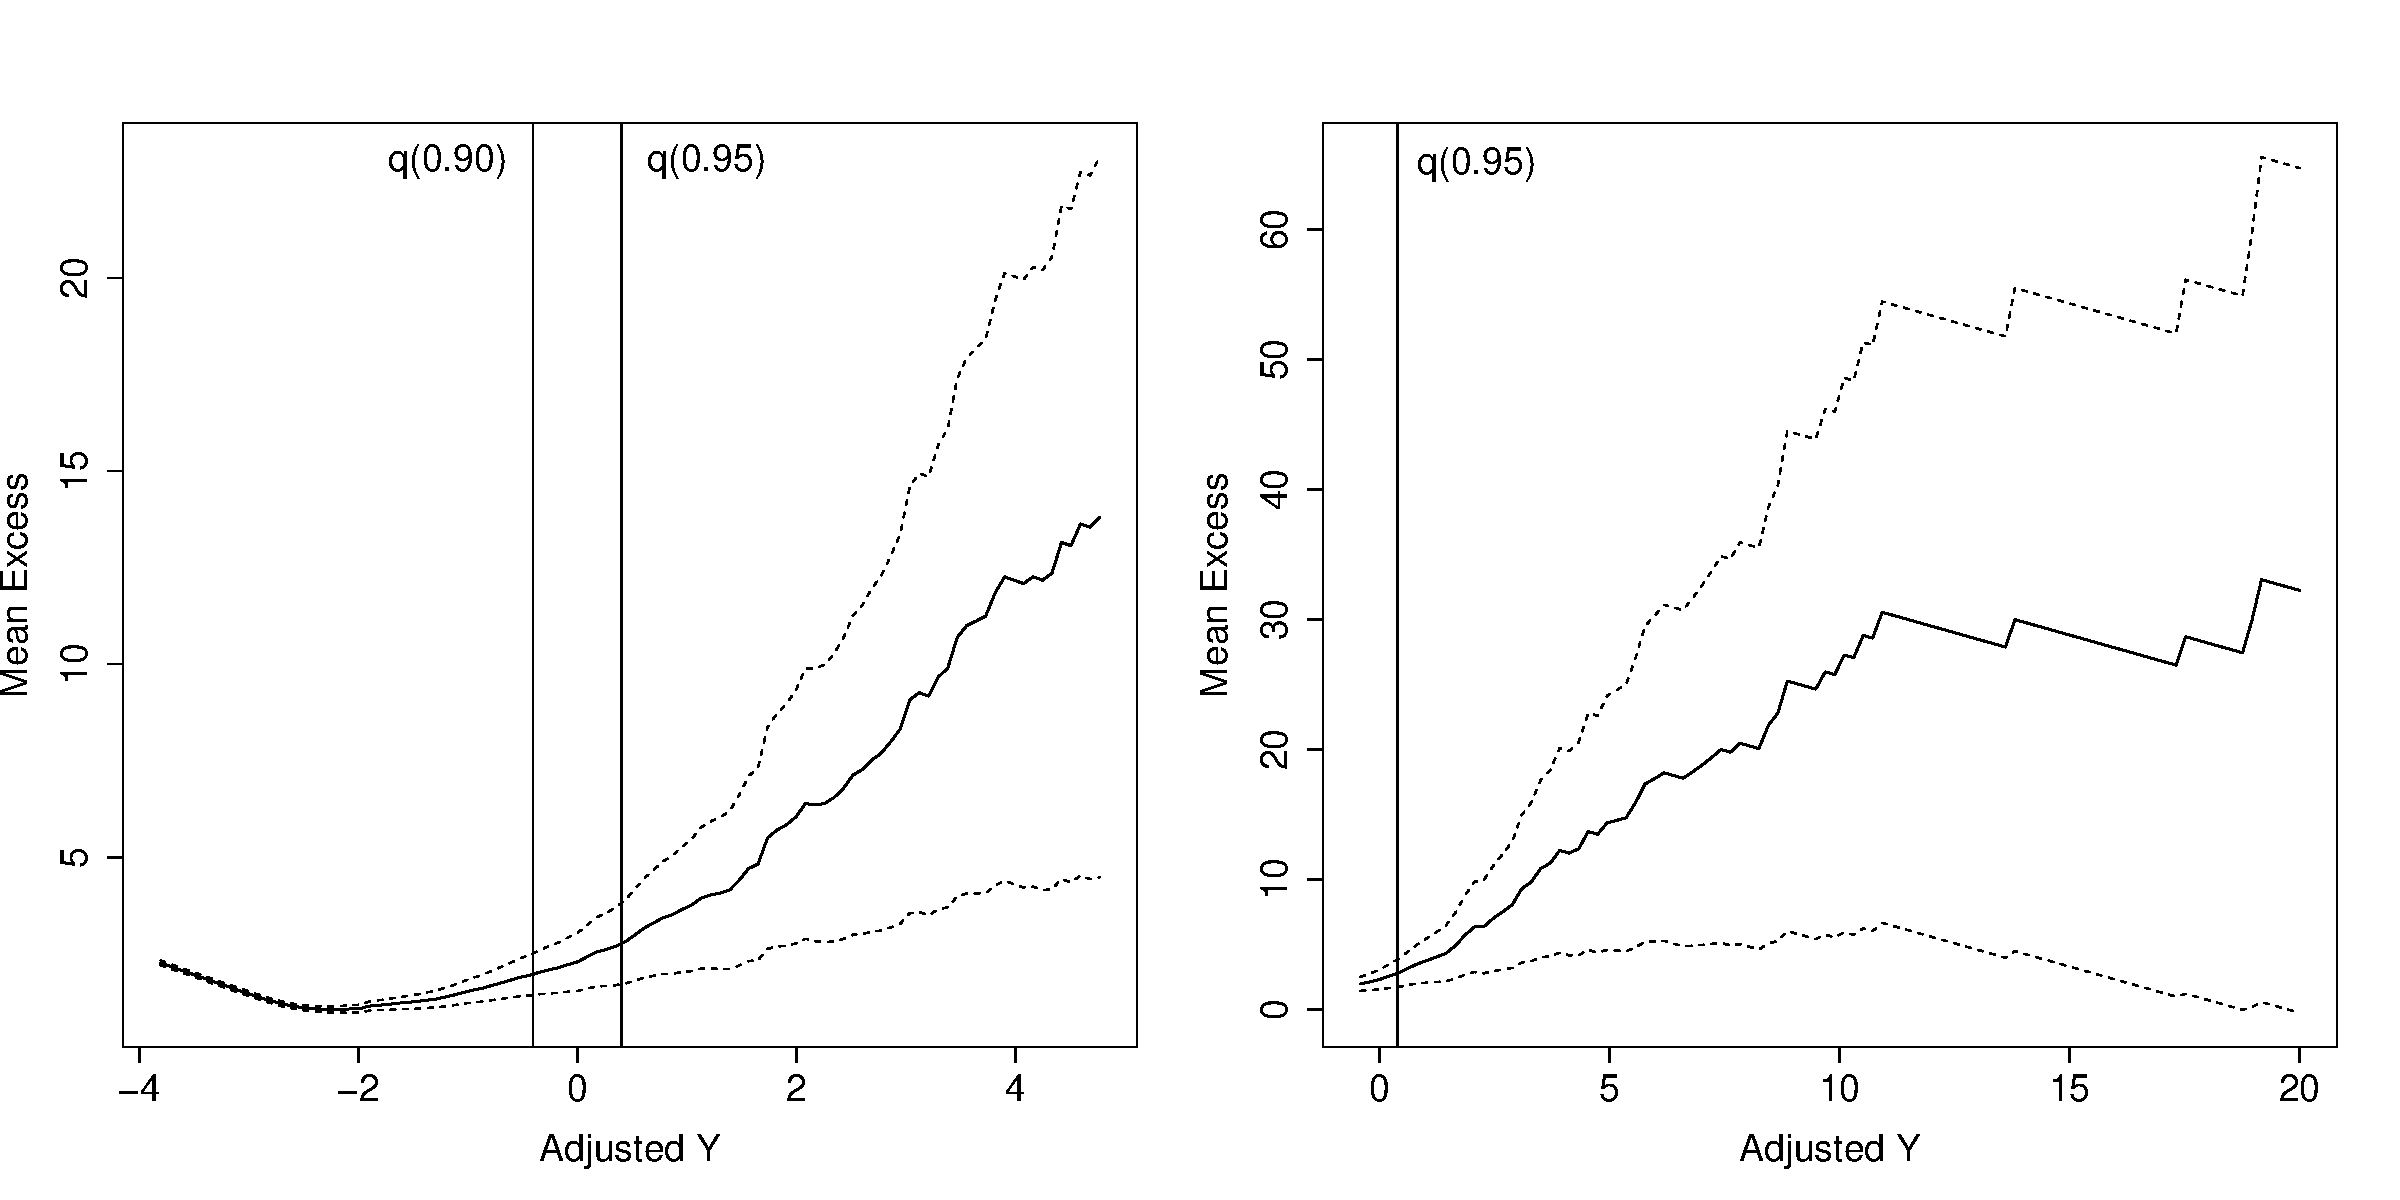
\includegraphics[width = \linewidth]{plots/fire-mrl-plots.pdf}  % markdown/eda/eda-plotting.R
  \caption{Mean residual plot for the data pooled across counties after standardizing using the county's median and interquartile range. The two panels show different ranges on the x-axis and include a vertical line at the sample 95th percentile.}
  \label{ebfig:mrlthresh}
\end{figure}

%\begin{figure}[htbp]
%  \centering
%  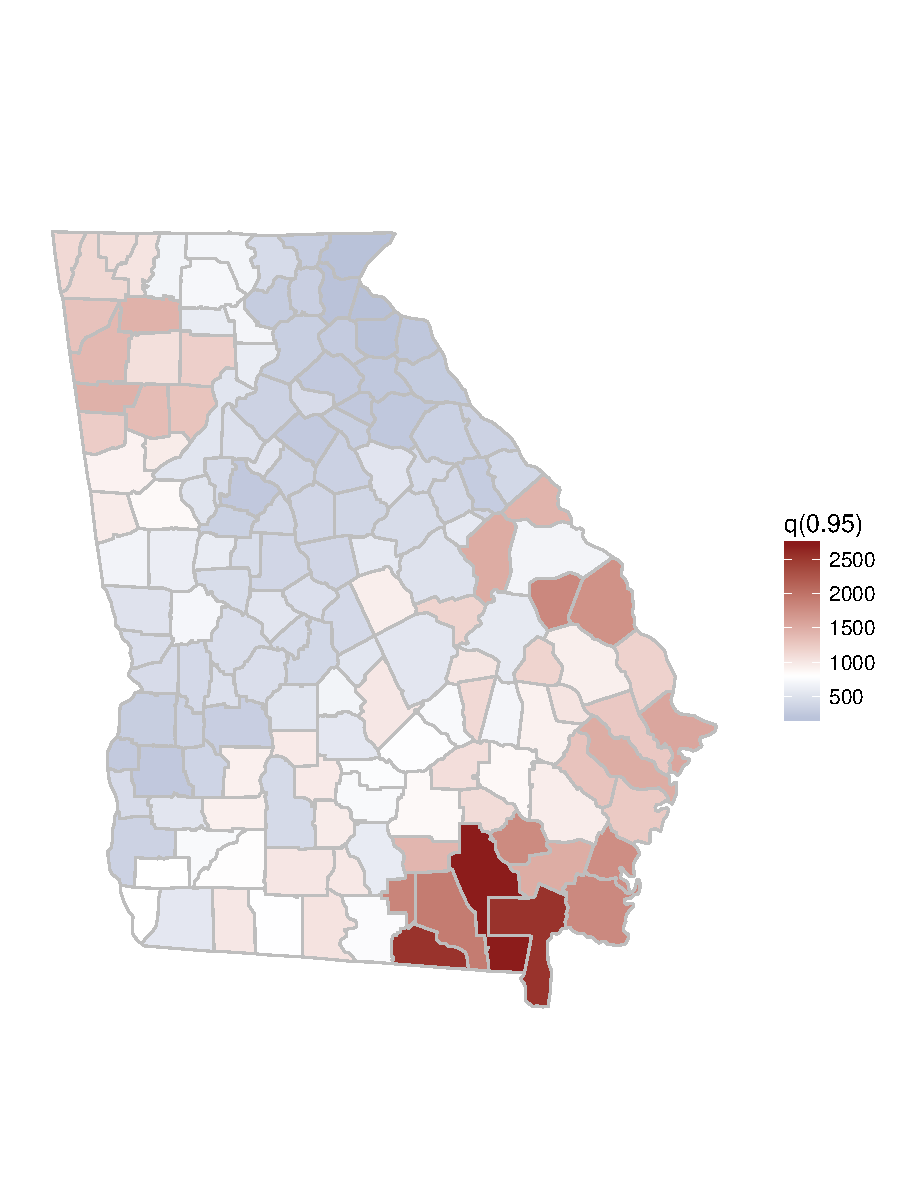
\includegraphics[width = 0.47\linewidth, trim = 0 10em 0 10em]{plots/fire-spatial-q95.pdf}
%  \caption{Spatially smoothed threshold values for each county.}
%  \label{fig:mrlthresh}
%\end{figure}

\subsection{Results for fire analysis}\label{ebs:results-fire}
We use 10-fold cross-validation to assess the predictive performance of a model.
For each method, we randomly select 90\% of the observations across counties and years to be used as a training set to fit the model.
The remaining 10\% of sites and years are withheld for testing model predictions.
To assess the predictions for the test set, we use quantile scores and Brier scores \hl{citation}.
The quantile score is given by \hl{give formula}.
The Brier score is given by \hl{give formula}.
For both of these methods, we use a negative orientation, so a lower score indicates a better fit.
The Brier and quantile scores for the fire analysis are given in \tref{ebtbl:firescores}.

Based on the Brier scores and quantiles scores, we run a full analysis using all of the data with $L = 35$.
Posterior summaries for each county's $\beta_\text{time}$ coefficient are given in \fref{ebfig:ebfpost} and \fref{ebfig:gskpost}.
These plots both seem to catch similar features with some differences particularly in the posterior distribution of the county-specific $\beta_{\mu, \text{time}}$.

\begin{table}[htbp]
\caption{Average Brier scores ($\times 100$) for selected thresholds and quantile scores for selected quantiles for fire analysis \hl{Need timings for L = 35, 40 to be added in}}
\label{ebtbl:firescores}
\centering
\small
  \begin{tabular}{lc|rr|rr|c}
  \multicolumn{2}{c}{  }& \multicolumn{2}{|c|}{Brier Scores ($\times 100$)} & \multicolumn{2}{|c|}{Quantile Scores} & Time (in hours)\\
  \hline
  & Process & $q(0.95)$ & $q(0.99)$ & $q(0.95)$ & $q(0.99)$\\
  \hline
  \multirow{2}{*}{L = 5}  & EBF & 5.640 & 2.265 & 135.685 & 80.471 & 1.1\\
                          & GSK & 5.726 & 2.301 & 134.419 & 78.639 & 1.1\\
  \hline
  \multirow{2}{*}{L = 10} & EBF & 5.329 & 2.130 & 127.313 & 75.974 & 1.8\\
                          & GSK & 5.311 & 2.142 & 127.593 & 75.123 & 1.9\\
  \hline
  \multirow{2}{*}{L = 15} & EBF & 4.997 & 2.043 & 128.277 & 68.946 & 2.7\\
                          & GSK & 4.907 & 2.034 & 124.537 & \textbf{59.266} & 2.7\\
  \hline
  \multirow{2}{*}{L = 20} & EBF & 4.930 & 2.036 & 122.394 & 66.413 & 3.7\\
                          & GSK & 4.864 & 2.043 & 121.145 & 62.172 & 3.7\\
  \hline
  \multirow{2}{*}{L = 25} & EBF & 4.776 & \textbf{1.920} & 116.944 & 61.704 & 4.8\\
                          & GSK & 4.740 & 1.921 & 113.872 & 59.524 & 4.7\\
  \hline
  \multirow{2}{*}{L = 30} & EBF & 4.745 & 1.923 & 114.878 & 62.020 & 5.9\\
                          & GSK & 4.719 & 1.936 & 114.918 & 61.905 & 5.7\\
  \hline
  \multirow{2}{*}{L = 35} & EBF & 4.761 & 1.920 & 115.696 & 62.581 & \\
                          & GSK & 4.767 & 1.933 & 114.026 & 60.805 & \\
  \hline
  \multirow{2}{*}{L = 40} & EBF & 4.722 & 1.935 & 115.213 & 62.039 & \\
                          & GSK & \textbf{4.716} & 1.921 & \textbf{113.362} & 60.300 & \\
  \hline
	\end{tabular}
\end{table}

\hl{We need a plot of the first 5 basis functions, and we also talked about the \% variability. I wasn't sure if this should be for $L = 35$ or a different number of knots.}

\begin{figure}  % markdown/fire-analysis/combine-tables.R
  \centering
  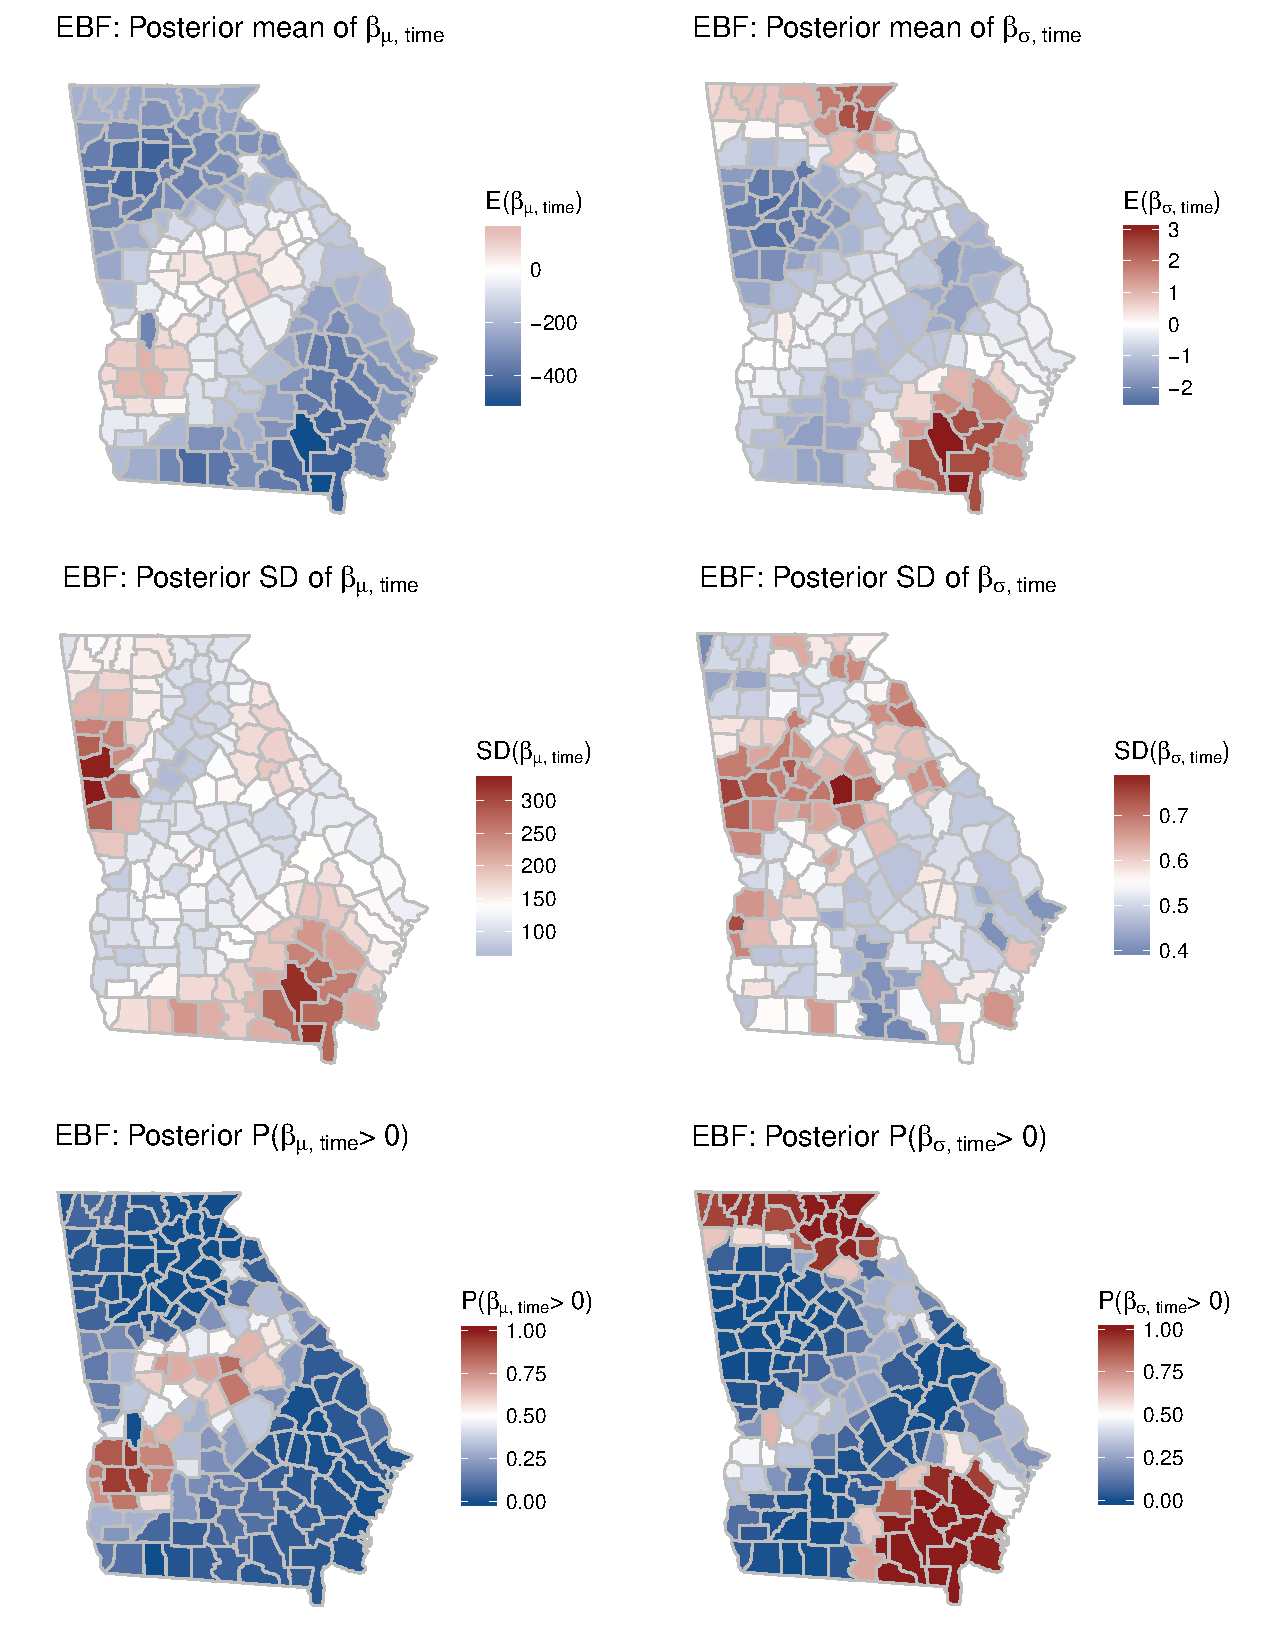
\includegraphics[width=\linewidth]{plots/ebf-post-betatime.pdf}
  \caption{Posterior summaries of $\beta_{\text{time}}$ when using EBF for the spatial process with $L = 35$.}
  \label{ebfig:ebfpost}
\end{figure}

\begin{figure}  % markdown/fire-analysis/combine-tables.R
  \centering
  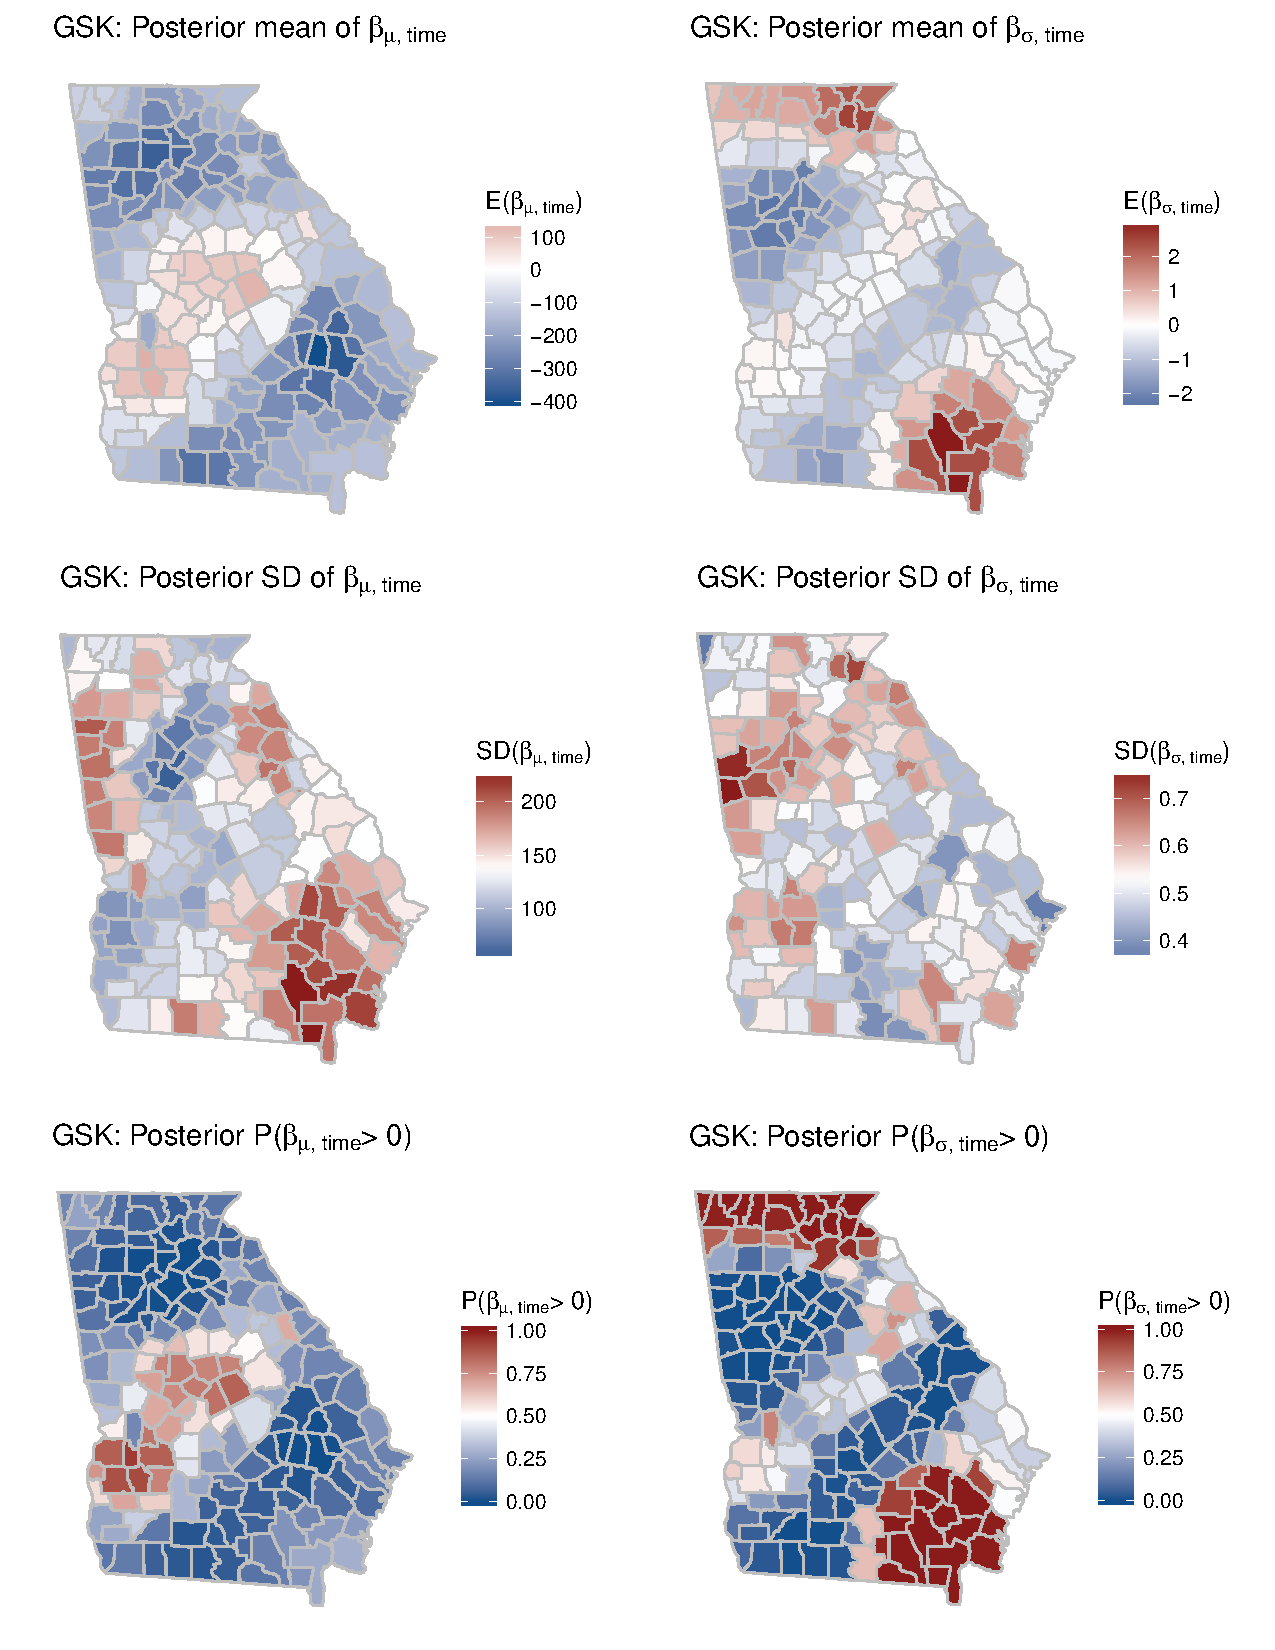
\includegraphics[width=\linewidth]{plots/gsk-post-betatime.pdf}
  \caption{Posterior summaries of $\beta_{\text{time}}$ when using GSK for the spatial process with $L = 35$.}
  \label{ebfig:gskpost}
\end{figure}

\begin{figure}  % markdown/fire-analysis/combine-tables.R
  \centering
  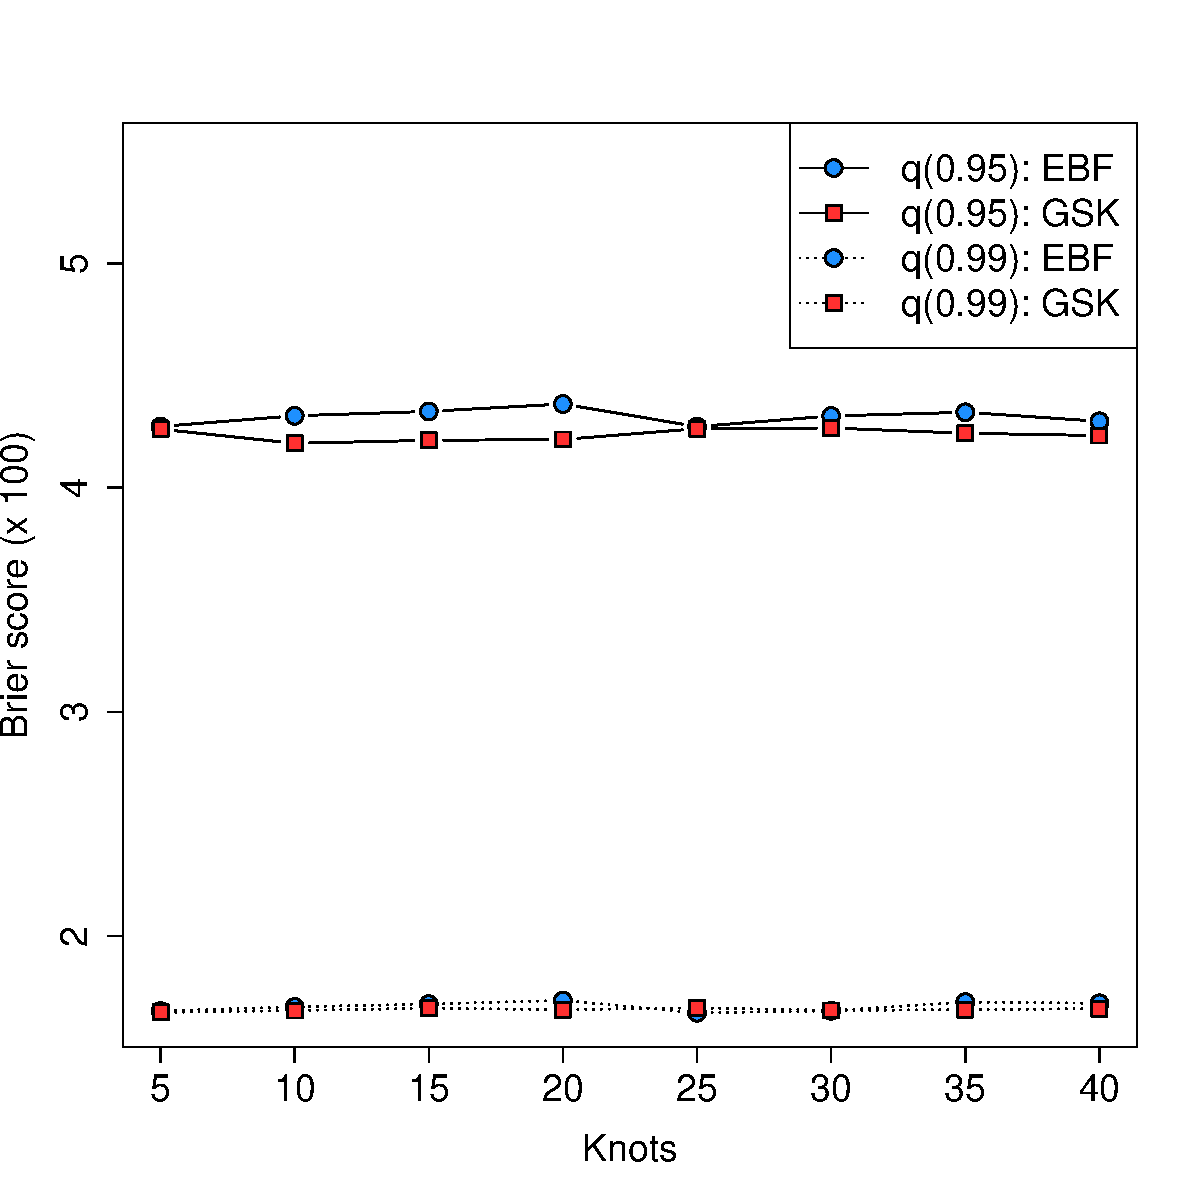
\includegraphics[width=0.47\linewidth]{plots/fire-bs}
  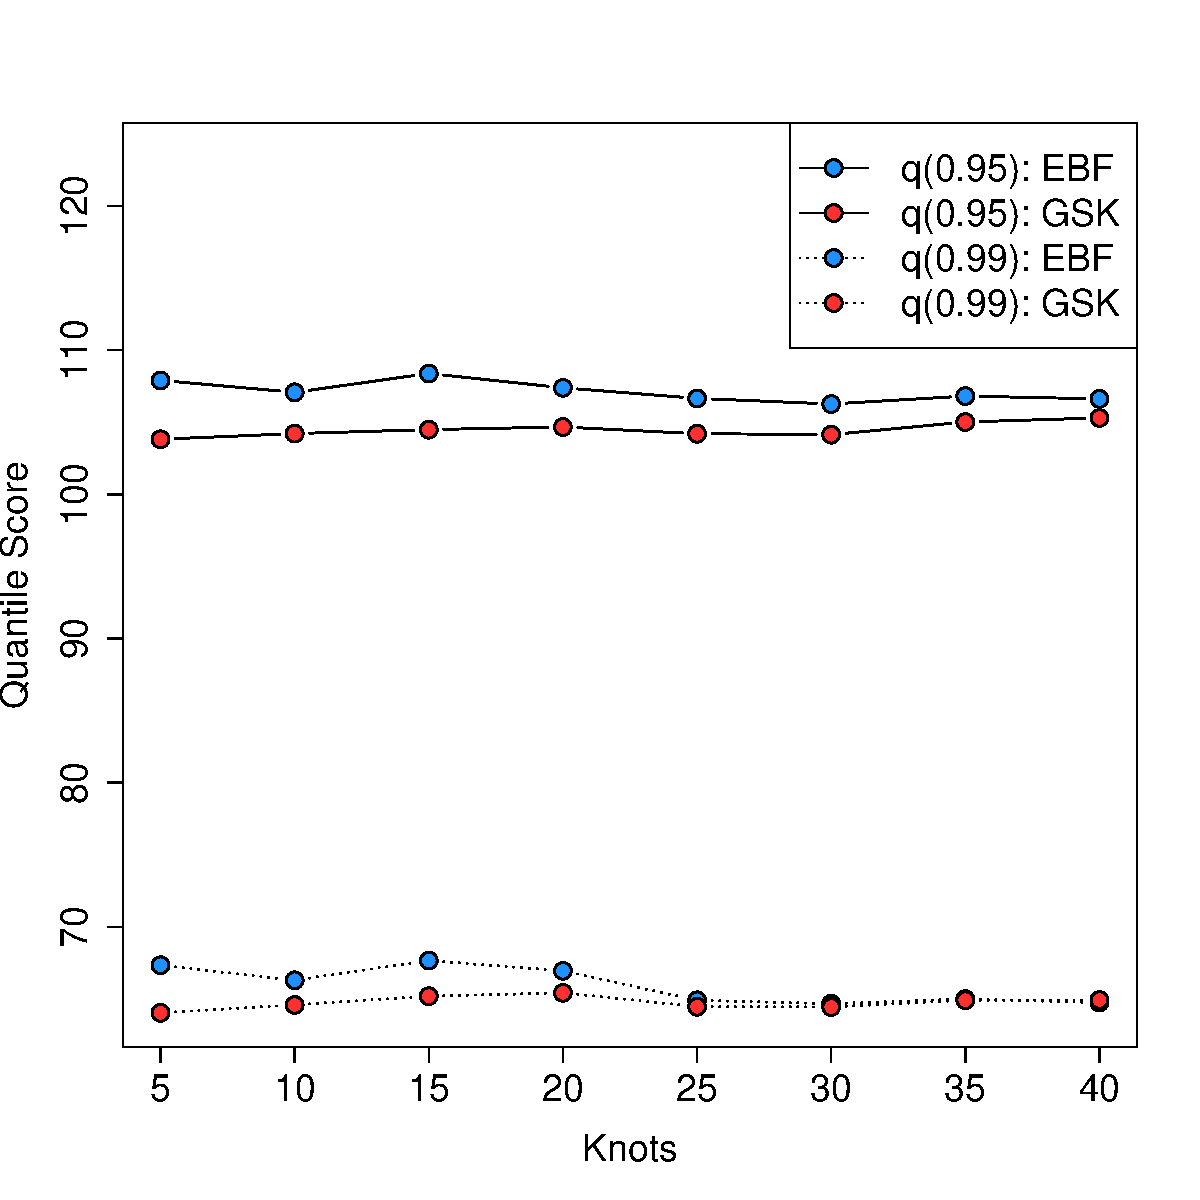
\includegraphics[width=0.47\linewidth]{plots/fire-qs}
  \caption{Average Brier score for exceeding q(0.95) and q(0.99) (left). Average Quantile score for exceeding q(0.95) and q(0.99) (right).}
  \label{fig:avgqscore}
\end{figure}

% \begin{figure}  % markdown/fire-analysis/combine-tables.R
% 	\centering
% 	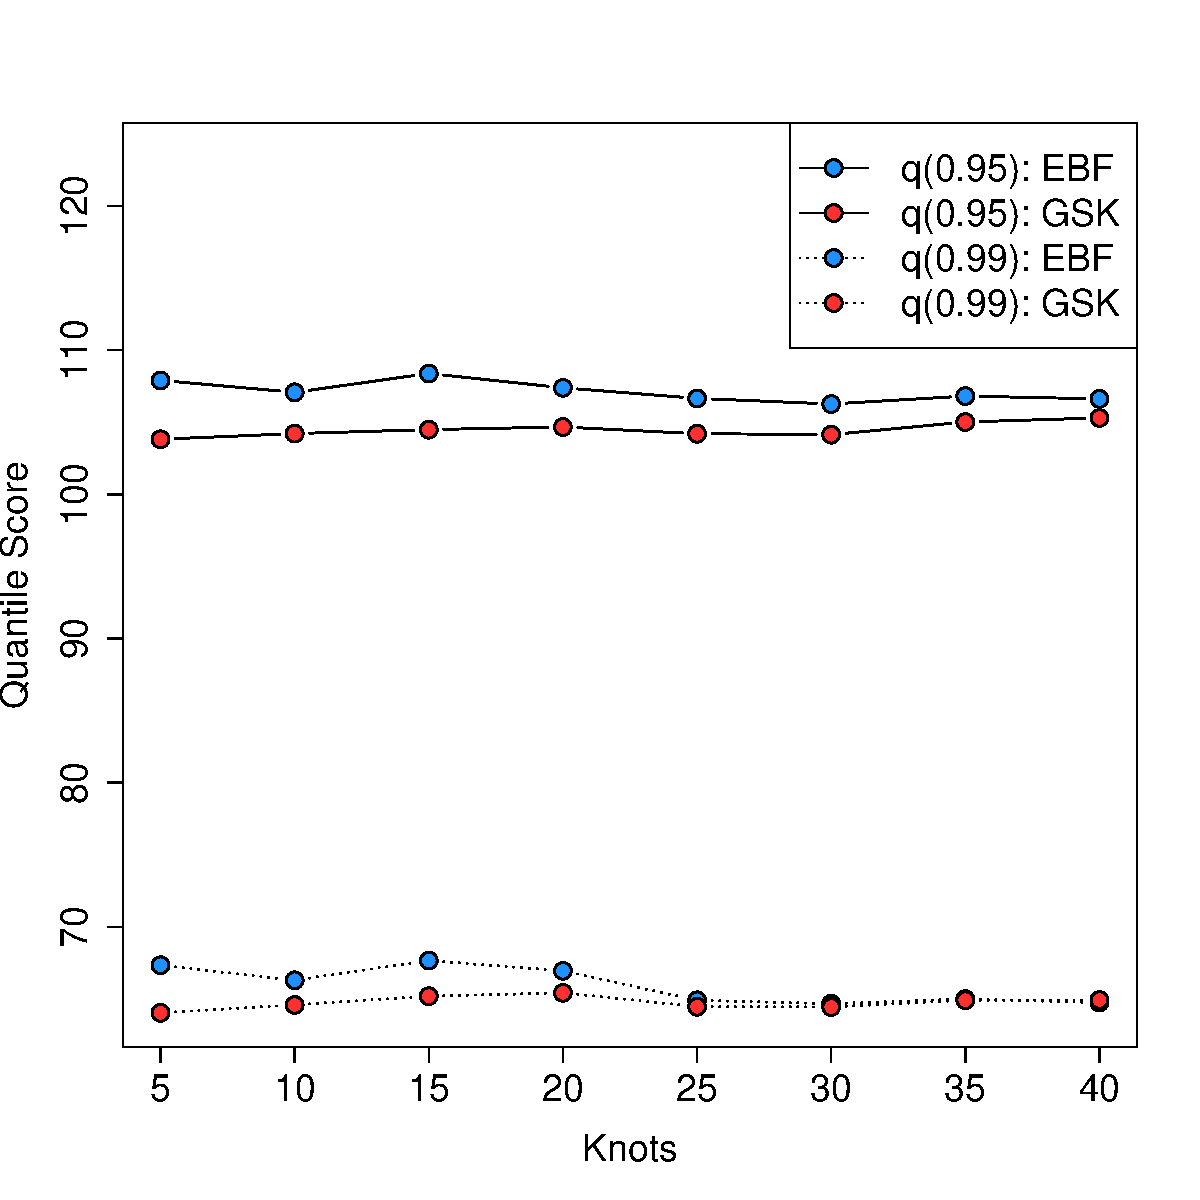
\includegraphics[width=\linewidth]{plots/fire-qs}
% 	\caption{Average quantile score for q(0.95) (left). Average quantile score for q(0.99) (right).}
%   \label{fig:avgqscore}
% \end{figure}

% \begin{figure}  % markdown/fire-analysis/combine-tables.R
% 	\centering
% 	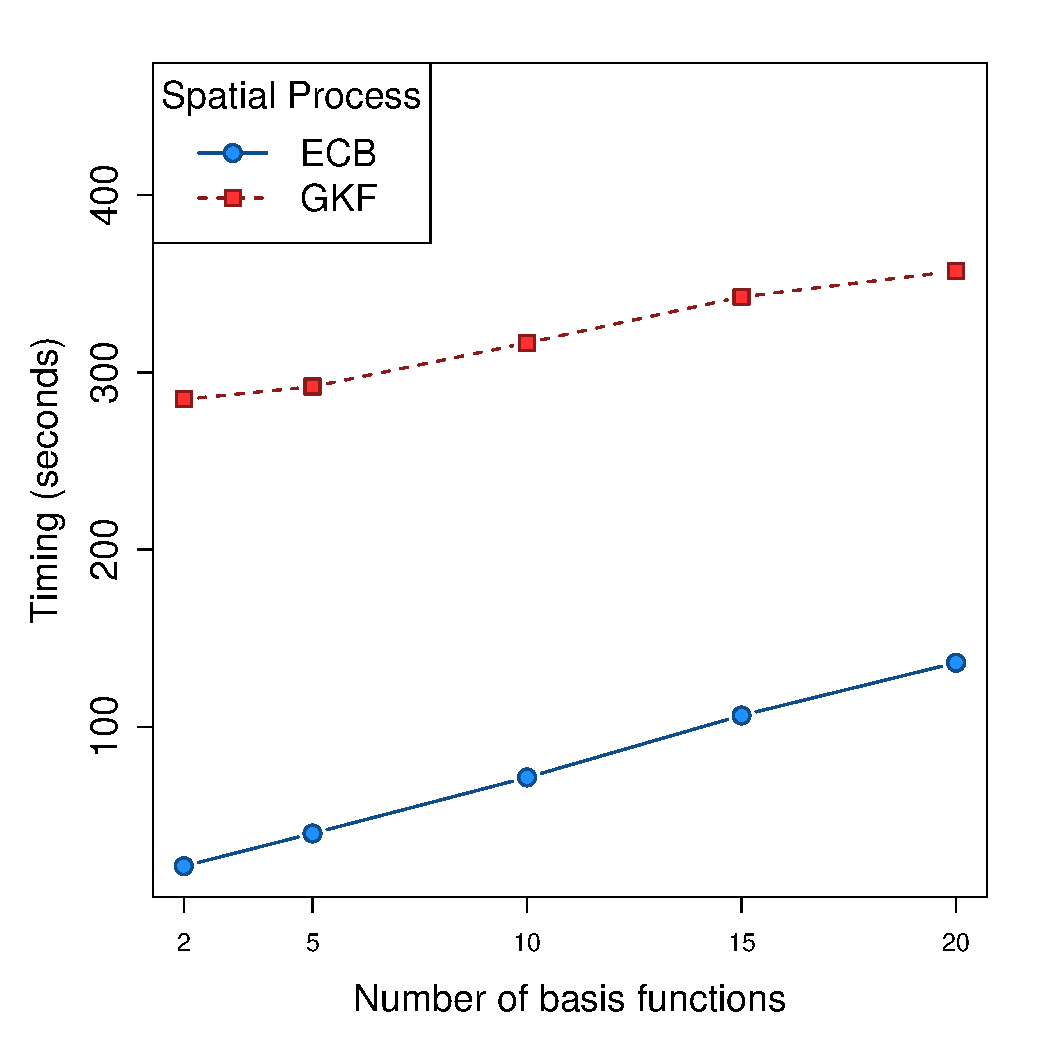
\includegraphics[width=0.47\linewidth]{plots/fire-timing}
% 	\caption{Timing comparison of basis functions to kernel functions for the spatial process (100 iterations)}
%   \label{fig:timingcompare}
% \end{figure}

Based upon the cross-validation results, we reran the full data analysis using $L = 15$ basis functions.
\hl{Figure here with panel of location \& scale: mean, sd, and P($\beta_t > 0$)}


\subsection{Model checking and sensitivity analysis}

\subsection{Analysis of annual precipitation}\label{ebs:precip}
We also conduct an analysis of the precipitation data presented in \citep{Reich2012}.
The data are climate model output from the North American Regional Climate Change Assessment Program (NARCCAP).
This data consists of $n_s = 697$ grid cells at a 50km resolution in the eastern US, and includes historical data (1969 -- 2000) as well as future conditions (2039 -- 2070).

\begin{figure}  % markdown/precipitation/cv-setup.R
  \centering
  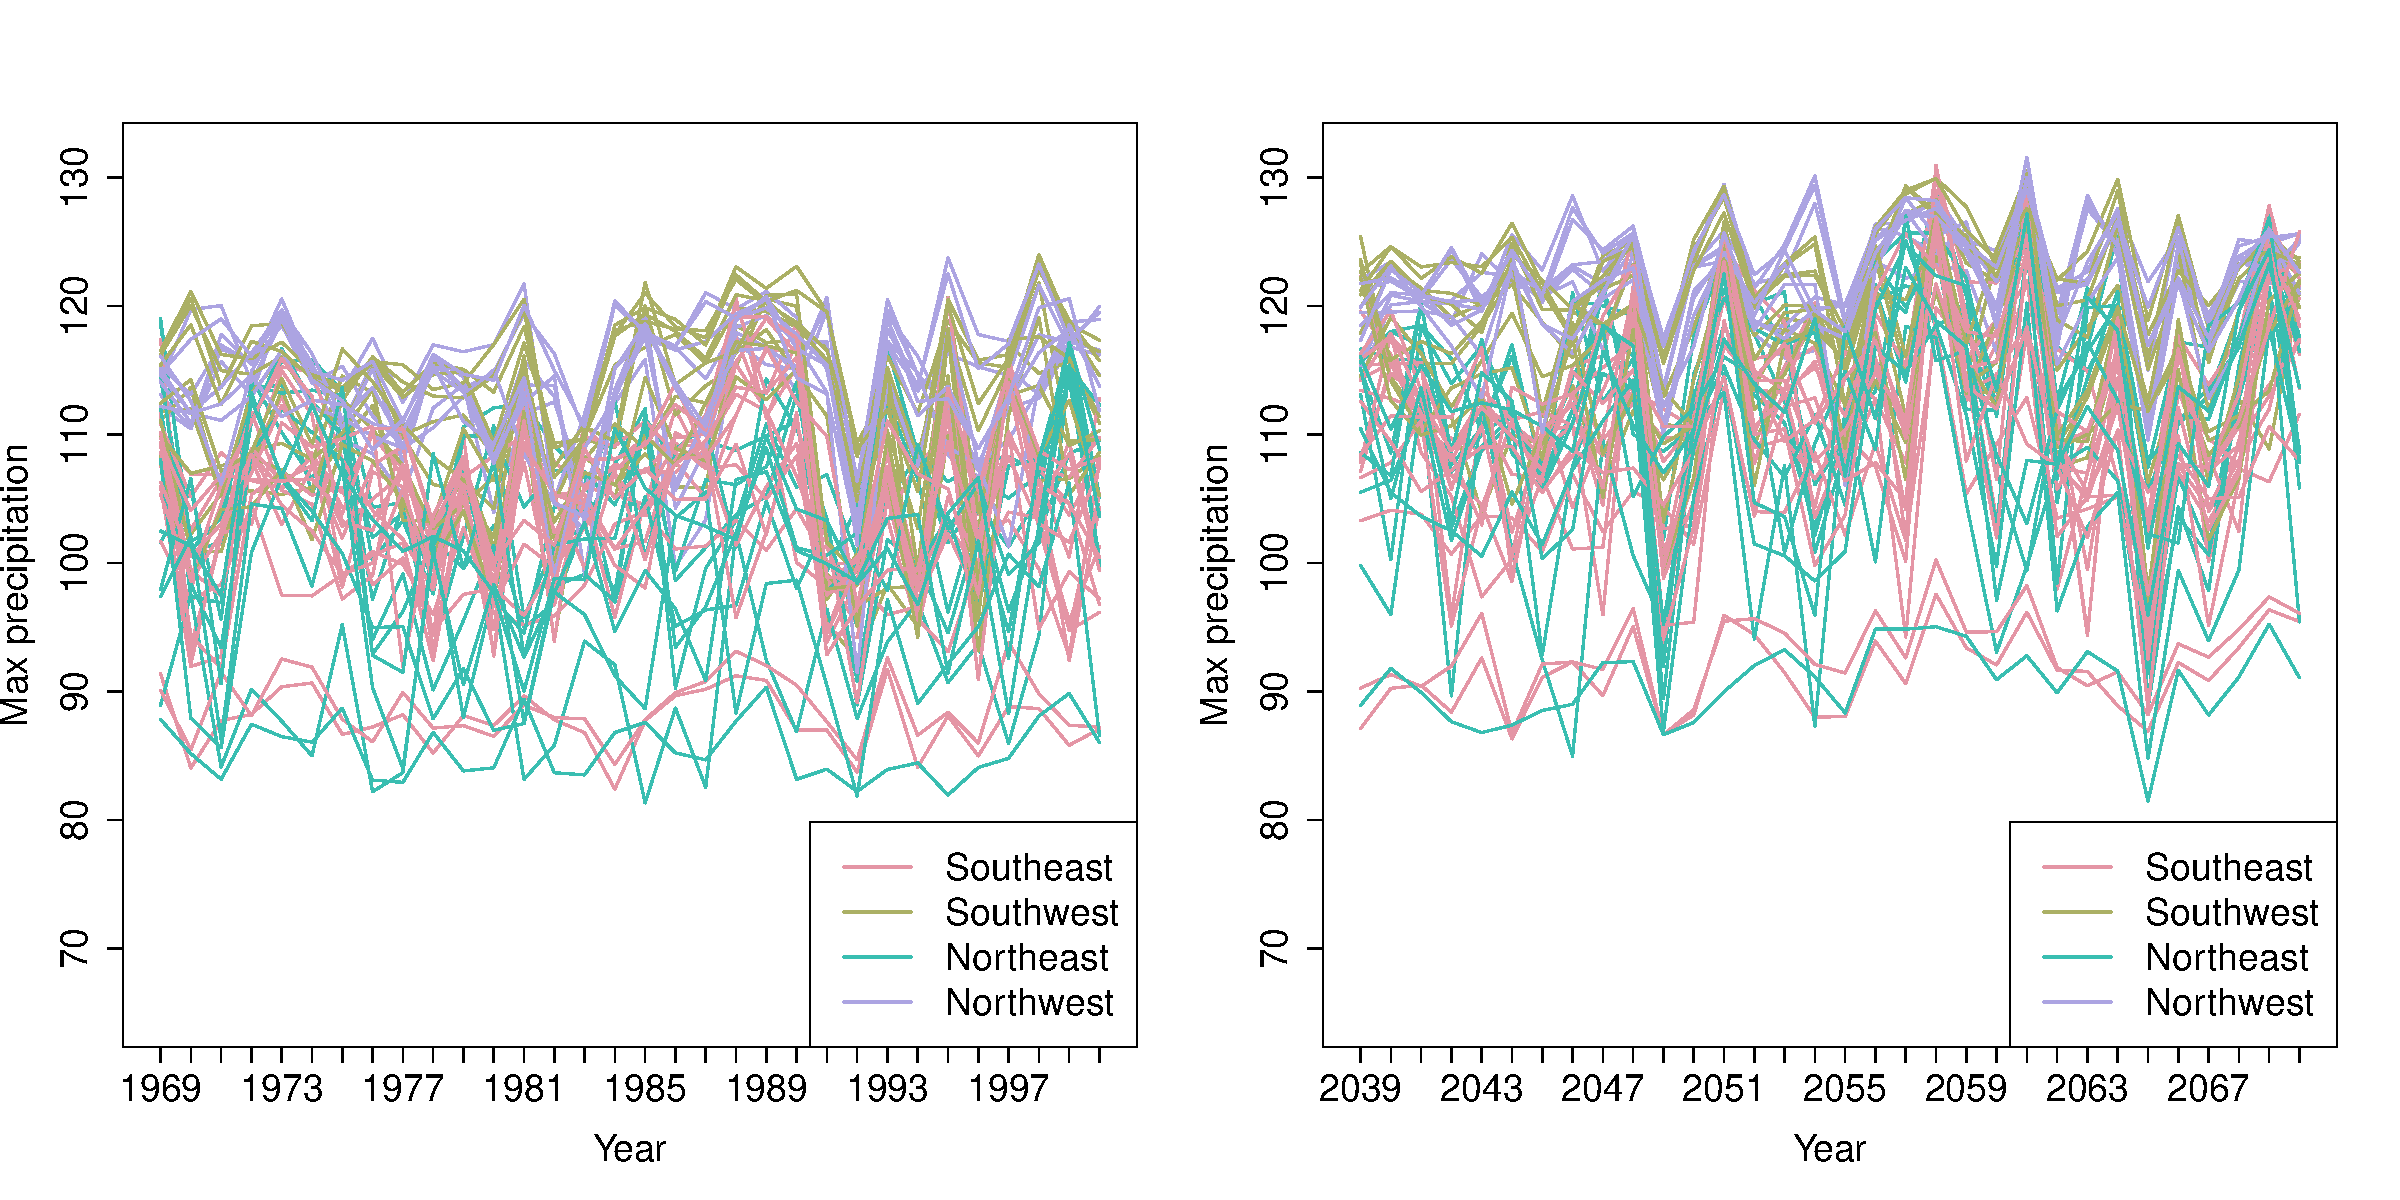
\includegraphics[width=\linewidth]{plots/precip-ts}
  \caption{Time series of yearly max precipitation for current (1969 -- 2000) (left). Time series of yearly max precipitation for future (2039 -- 2070) (right).}
  \label{ebf:tsprecip}
\end{figure}

\hl{Include figures of locations of grid cells}

\subsection{Results for precipitation analysis}\label{ebs:results-precip}

\begin{figure}  % markdown/precipitation/combine-tables.R
  \centering
  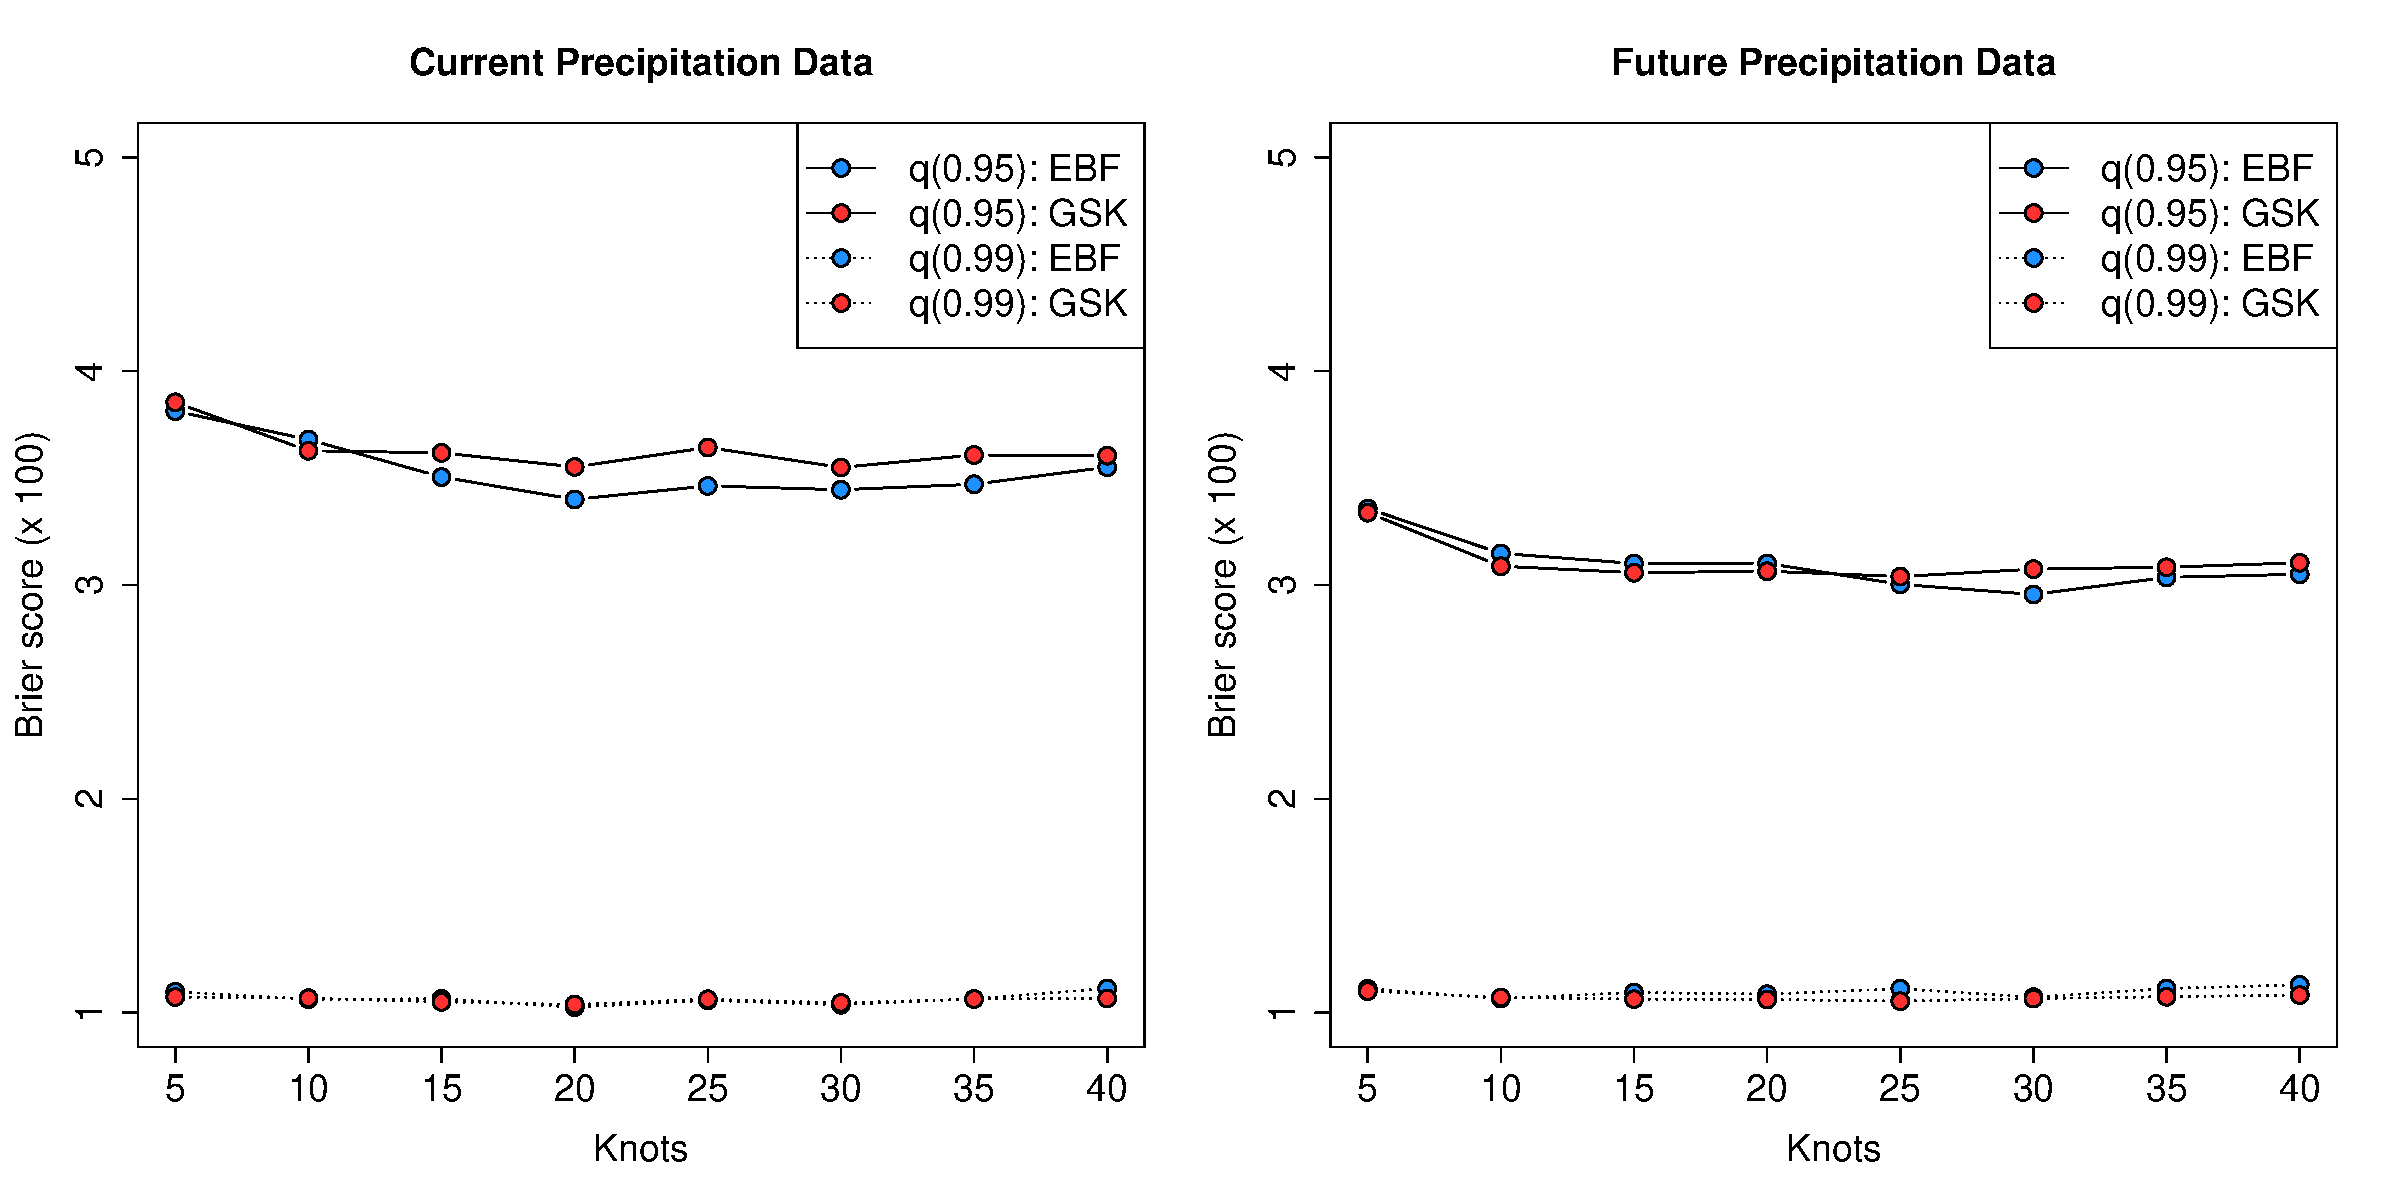
\includegraphics[width=\linewidth]{plots/precip-bs.pdf}
  \caption{Brier scores for current and future precipitation analysis.}
  \label{ebfig:precip-bs}
\end{figure}

\begin{figure}  % markdown/precipitation/combine-tables.R
  \centering
  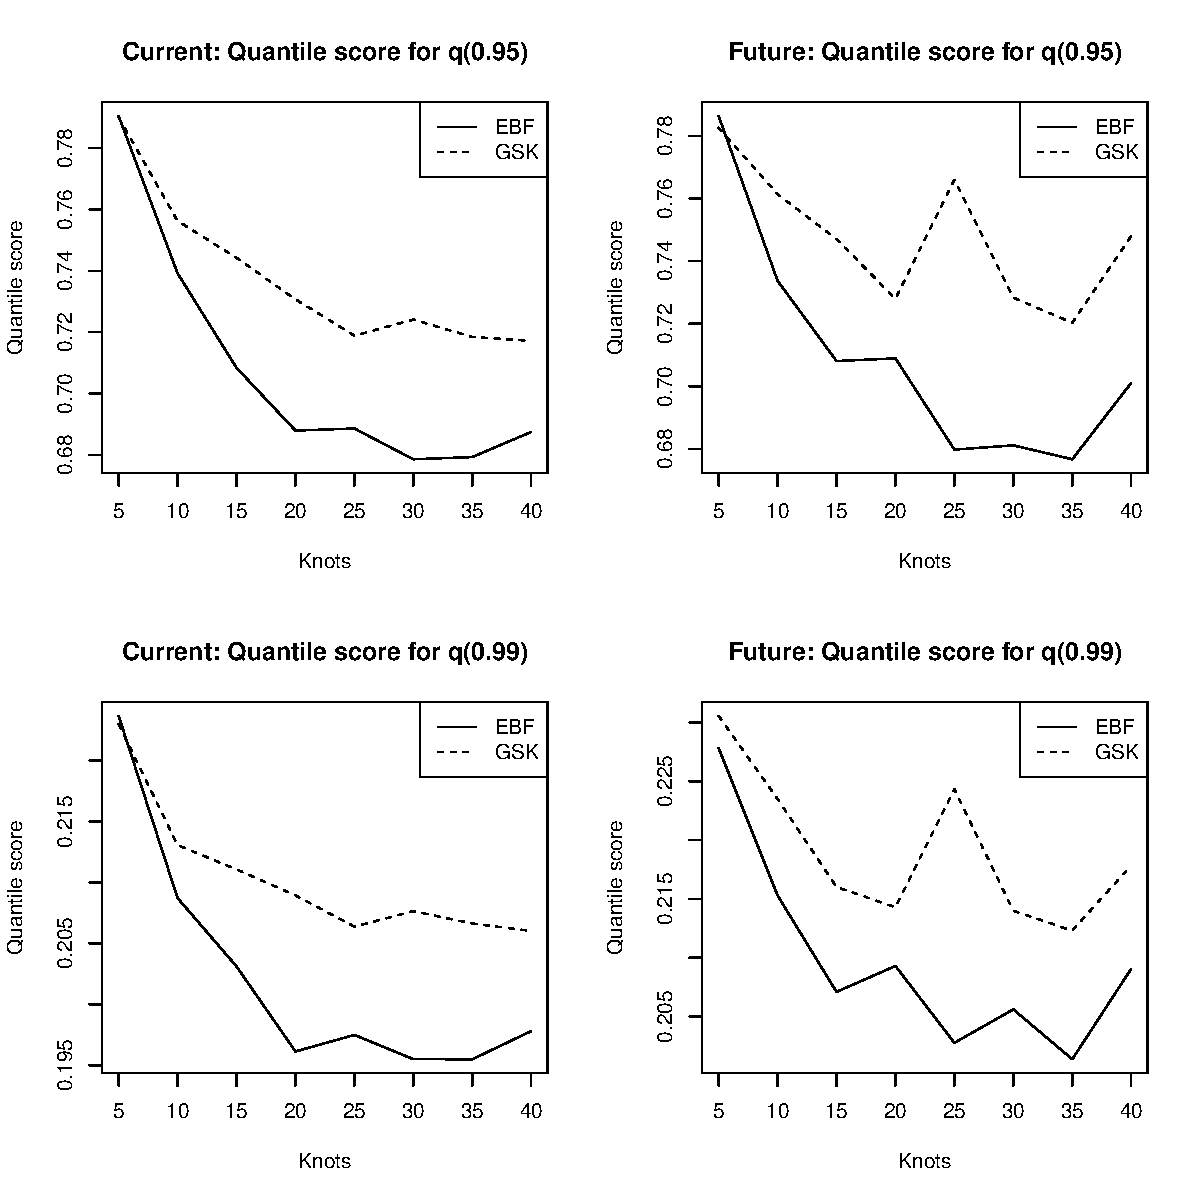
\includegraphics[width=\linewidth]{plots/precip-qs.pdf}
  \caption{Quantile scores for current and future precipitation analysis.}
  \label{ebfig:precip-qs}
\end{figure}

\begin{figure}  % markdown/precipitation/combine-tables.R
  \centering
  \includegraphics[width=\linewidth]{plots/precip-post-time.pdf}
  \caption{Posterior distributions for $\beta_{\text{time}}$ for $\mu$ (left) and $\log(\sigma)$ (right).}
  \label{ebfig:precip-qs}
\end{figure}

\section{Conclusions}\label{ebs:con}

\section*{Acknowledgements}
The authors would like to acknowledge Dan Cooley for his helpful suggestions on the manuscript.

\section*{A.1 Extreme value distributions}
Define (1) GEV density f and CDF F; (2) PS pdf  and the grid approximation to the integral.

\section*{A.2 Gradient for $\beta$}

\begin{singlespace}
\bibliographystyle{rss}
\bibliography{library}
\end{singlespace}

\end{document}




